%  LaTeX support: latex@mdpi.com 
%  In case you need support, please attach all files that are necessary for compiling as well as the log file, and specify the details of your LaTeX setup (which operating system and LaTeX version / tools you are using).

%=================================================================
\documentclass[remotesensing,article,submit,moreauthors,pdftex]{Definitions/mdpi} 

% If you would like to post an early version of this manuscript as a preprint, you may use preprint as the journal and change 'submit' to 'accept'. The document class line would be, e.g., \documentclass[preprints,article,accept,moreauthors,pdftex]{mdpi}. This is especially recommended for submission to arXiv, where line numbers should be removed before posting. For preprints.org, the editorial staff will make this change immediately prior to posting.

%--------------------
% Class Options:
%--------------------
%----------
% journal
%----------
% Choose between the following MDPI journals:
% acoustics, actuators, addictions, admsci, aerospace, agriculture, agriengineering, agronomy, algorithms, animals, antibiotics, antibodies, antioxidants, applsci, arts, asc, asi, atmosphere, atoms, axioms, batteries, bdcc, behavsci , beverages, bioengineering, biology, biomedicines, biomimetics, biomolecules, biosensors, brainsci , buildings, cancers, carbon , catalysts, cells, ceramics, challenges, chemengineering, chemistry, chemosensors, children, cleantechnol, climate, clockssleep, cmd, coatings, colloids, computation, computers, condensedmatter, cosmetics, cryptography, crystals, dairy, data, dentistry, designs , diagnostics, diseases, diversity, drones, econometrics, economies, education, ejihpe, electrochem, electronics, energies, entropy, environments, epigenomes, est, fermentation, fibers, fire, fishes, fluids, foods, forecasting, forests, fractalfract, futureinternet, futurephys, galaxies, games, gastrointestdisord, gels, genealogy, genes, geohazards, geosciences, geriatrics, hazardousmatters, healthcare, heritage, highthroughput, horticulturae, humanities, hydrology, ijerph, ijfs, ijgi, ijms, ijns, ijtpp, informatics, information, infrastructures, inorganics, insects, instruments, inventions, iot, j, jcdd, jcm, jcp, jcs, jdb, jfb, jfmk, jimaging, jintelligence, jlpea, jmmp, jmse, jnt, jof, joitmc, jpm, jrfm, jsan, land, languages, laws, life, literature, logistics, lubricants, machines, magnetochemistry, make, marinedrugs, materials, mathematics, mca, medicina, medicines, medsci, membranes, metabolites, metals, microarrays, micromachines, microorganisms, minerals, modelling, molbank, molecules, mps, mti, nanomaterials, ncrna, neuroglia, nitrogen, notspecified, nutrients, ohbm, optics, particles, pathogens, pharmaceuticals, pharmaceutics, pharmacy, philosophies, photonics, physics, plants, plasma, polymers, polysaccharides, preprints , proceedings, processes, proteomes, psych, publications, quantumrep, quaternary, qubs, reactions, recycling, religions, remotesensing, reports, resources, risks, robotics, safety, sci, scipharm, sensors, separations, sexes, signals, sinusitis, smartcities, sna, societies, socsci, soilsystems, sports, standards, stats, surfaces, surgeries, sustainability, symmetry, systems, technologies, test, toxics, toxins, tropicalmed, universe, urbansci, vaccines, vehicles, vetsci, vibration, viruses, vision, water, wem, wevj

%---------
% article
%---------
% The default type of manuscript is "article", but can be replaced by: 
% abstract, addendum, article, benchmark, book, bookreview, briefreport, casereport, changes, comment, commentary, communication, conceptpaper, conferenceproceedings, correction, conferencereport, expressionofconcern, extendedabstract, meetingreport, creative, datadescriptor, discussion, editorial, essay, erratum, hypothesis, interestingimages, letter, meetingreport, newbookreceived, obituary, opinion, projectreport, reply, retraction, review, perspective, protocol, shortnote, supfile, technicalnote, viewpoint
% supfile = supplementary materials

%----------
% submit
%----------
% The class option "submit" will be changed to "accept" by the Editorial Office when the paper is accepted. This will only make changes to the frontpage (e.g., the logo of the journal will get visible), the headings, and the copyright information. Also, line numbering will be removed. Journal info and pagination for accepted papers will also be assigned by the Editorial Office.

%------------------
% moreauthors
%------------------
% If there is only one author the class option oneauthor should be used. Otherwise use the class option moreauthors.

%---------
% pdftex
%---------
% The option pdftex is for use with pdfLaTeX. If eps figures are used, remove the option pdftex and use LaTeX and dvi2pdf.

%=================================================================
\firstpage{1} 
\makeatletter 
\setcounter{page}{\@firstpage} 
\makeatother
\pubvolume{xx}
\issuenum{1}
\articlenumber{5}
\pubyear{2019}
\copyrightyear{2019}
%\externaleditor{Academic Editor: name}
\history{Received: date; Accepted: date; Published: date}
\graphicspath{{../../Dissertacao/figuras/}}  % AAB inserido - caminho das figuras
%\ifCLASSOPTIONcompsoc                        % AAB inseri#do#
%\usepackage[caption=false,font=normalsize,labelfont=sf,textfont=sf]{subfig}
%\else
\usepackage[caption=false,font=footnotesize]{subfig}
%\fi
\usepackage{booktabs}                   % AAB inserido
\usepackage{siunitx}                    % AAB inserido
\usepackage{rotating}                   % AAB inserido
\usepackage[utf8]{inputenc}             % AAB inserido
\usepackage{bm,bbm}                     % AAB inserido
%\usepackage{biblatex}                    % AAB inserido
%================================
% Add packages and commands here. The following packages are loaded in our class file: fontenc, calc, indentfirst, fancyhdr, graphicx, lastpage, ifthen, lineno, float, amsmath, setspace, enumitem, mathpazo, booktabs, titlesec, etoolbox, amsthm, hyphenat, natbib, hyperref, footmisc, geometry, caption, url, mdframed, tabto, soul, multirow, microtype, tikz

%=================================================================
%% Please use the following mathematics environments: Theorem, Lemma, Corollary, Proposition, Characterization, Property, Problem, Example, ExamplesandDefinitions, Hypothesis, Remark, Definition, Notation, Assumption
%% For proofs, please use the proof environment (the amsthm package is loaded by the MDPI class).

%=================================================================
% Full title of the paper (Capitalized)
%\Title{Quantifying the Information Content of Intensity SAR Imagery for Edge Detection}    % ACF inserido
\Title{Edge Location from Partial Information in PolSAR Imagery}     % AAB inserido

% Author Orchid ID: enter ID or remove command
\newcommand{\orcidauthorA}{000-002-6830-1067}
\newcommand{\orcidauthorB}{0000-0002-8002-5341}
\newcommand{\orcidauthorC}{0000-0001-8479-9128}

% Authors, for the paper (add full first names)
\Author{Anderson Adaime Borba $^{1,3,\dagger}$\orcidA{}, Alejandro C.\ Frery $^{2,\dagger}$\orcidB{} 
and Maur\'icio Marengoni $^{3,\dagger}$*\orcidC{}}

% Authors, for metadata in PDF
\AuthorNames{Anderson Adaime Borba, Alejandro C. Frery and Mauricio Marengoni}

% Affiliations / Addresses (Add [1] after \address if there is only one affiliation.)
\address{%
$^{1}$ IBMEC-SP, S\~ao Paulo, Brazil;anderson.borba@ibmec.edu.br\\
$^{2}$ Laborat\'orio de Computa\c c\~ao Cient\'ifica e An\'alise Num\'erica, Universidade Federal de Alagoas,
Maceió, Brazil; acfrery@laccan.ufal.br\\
$^{3}$ Dept.\ Engenharia El\'etrica e Computa\c c\~ao, Universidade Presbiteriana Mackenzie, S\~ao Paulo, Brazil; mmarengoni@mackenzie.br}

% Contact information of the corresponding author
\corres{Correspondence: mmarengoni@mackenzie.br}

% Current address and/or shared authorship
\firstnote{These authors contributed equally to this work.}
% The commands \thirdnote{} till \eighthnote{} are available for further notes

%\simplesumm{} % Simple summary

%\conference{} % An extended version of a conference paper

% Abstract (Do not insert blank lines, i.e. \\) 
\abstract{This work studies cost-effective techniques for edge detection using intensity SAR data.
The approach consists in using statistical models for obtaining evidences, and then fusing such evidences.
We quantify the amount of information each combination of bands brings, and compute the computational cost of using each model.
}

% Keywords
\keyword{Synthetic Aperture Radar (SAR); Edge Detection; Information Fusion; Statistical Models.}

% The fields PACS, MSC, and JEL may be left empty or commented out if not applicable
%\PACS{J0101}
%\MSC{}
%\JEL{}

%%%%%%%%%%%%%%%%%%%%%%%%%%%%%%%%%%%%%%%%%%
% Only for the journal Diversity
%\LSID{\url{http://}}

%%%%%%%%%%%%%%%%%%%%%%%%%%%%%%%%%%%%%%%%%%
% Only for the journal Applied Sciences:
%\featuredapplication{Authors are encouraged to provide a concise description of the specific application or a potential application of the work. This section is not mandatory.}
%%%%%%%%%%%%%%%%%%%%%%%%%%%%%%%%%%%%%%%%%%

%%%%%%%%%%%%%%%%%%%%%%%%%%%%%%%%%%%%%%%%%%
% Only for the journal Data:
%\dataset{DOI number or link to the deposited data set in cases where the data set is published or set to be published separately. If the data set is submitted and will be published as a supplement to this paper in the journal Data, this field will be filled by the editors of the journal. In this case, please make sure to submit the data set as a supplement when entering your manuscript into our manuscript editorial system.}

%\datasetlicense{license under which the data set is made available (CC0, CC-BY, CC-BY-SA, CC-BY-NC, etc.)}

%%%%%%%%%%%%%%%%%%%%%%%%%%%%%%%%%%%%%%%%%%
% Only for the journal Toxins
%\keycontribution{The breakthroughs or highlights of the manuscript. Authors can write one or two sentences to describe the most important part of the paper.}

%\setcounter{secnumdepth}{4}
\makeindex                      % AAB inserido
%%%%%%%%%%%%%%%%%%%%%%%%%%%%%%%%%%%%%%%%%%
\begin{document}
%%%%%%%%%%%%%%%%%%%%%%%%%%%%%%%%%%%%%%%%%%

%%%%%%%%%%%%%%%%%%%%%%%%%%%%%%%%%%%%%%%%%%
%\setcounter{section}{-1} %% Remove this when starting to work on the template.
%\section{How to Use this Template}
%The template details the sections that can be used in a manuscript. Note that the order and names of article sections may differ from the requirements of the journal (e.g., the positioning of the Materials and Methods section). Please check the instructions for authors page of the journal to verify the correct order and names. For any questions, please contact the editorial office of the journal or support@mdpi.com. For LaTeX related questions please contact latex@mdpi.com.
%The order of the section titles is: Introduction, Materials and Methods, Results, Discussion, Conclusions for these journals: aerospace,algorithms,antibodies,antioxidants,atmosphere,axioms,biomedicines,carbon,crystals,designs,diagnostics,environments,fermentation,fluids,forests,fractalfract,informatics,information,inventions,jfmk,jrfm,lubricants,neonatalscreening,neuroglia,particles,pharmaceutics,polymers,processes,technologies,viruses,vision


\section{Introduction}
\cite{lee}
\section{Methodology}
\subsection{Sharp Edge Model}
\subsection{Models}
\subsubsection{Fully PolSAR}
\subsubsection{Marginal Models}
%Numbered lists can be added as follows:
\begin{enumerate}[leftmargin=*,labelsep=4.9mm]
	\item Univariate Distribution
		\begin{enumerate}[leftmargin=*,labelsep=4.9mm]
		\item	Gamma -  
			We assume that the distribution of each intensity channel is a 
			Gamma law with probability density function
			\begin{equation}
			f_Z(z;\mu,L)=\frac{L^{L}z^{L-1}}{\mu^{L}\Gamma(L)} \exp\big\{-Lz/\mu\big\},\quad z>0,
			\label{func_dens_uni_gamma}
			\end{equation}
			where $L>0$ (rather than $L\geq1$ to allow for flexibility), and $\mu>0$ is the mean.

			Given the sample $\bm z = (z_1,\dots,z_n)$, the reduced log-likelihood of this model is
			\begin{equation}
			\ell(\bm z; L,\mu) = n \big[L\ln (L / \mu) - \ln \Gamma(L)\big]+L \sum_{k=1}^{n}\ln z_k -\frac{L}{\mu}\sum_{k=1}^{n}z_k.
			\label{eq:LogLikelihoodGamma_2_param}
			\end{equation}
			With the multi-look L fixed, 	
			\begin{equation}
			\ell(\bm z; \mu) = -n\ln (\mu) - \frac{1}{\mu}\sum_{k=1}^{n}z_k.
			\label{eq:LogLikelihoodGamma_1_param}
			\end{equation}
			We obtain $\widehat \mu$, the maximum likelihood estimator (MLE) of $\mu$ based on $\bm z$, by 					maximizing~\eqref{eq:LogLikelihoodGamma_1_param} with the BFGS method implemented in the \texttt{maxLik} package~\cite{ht}. Note that $\mu=\sum_{k=1}^{n}z_k$ is a maximum candidate.  
		\item	Product of Intensities
		\item	Ratio of Intensities
		\end{enumerate}
	\item Bivariate Distribution
	\item Trivariate Distribution
	\item Parameter Estimation
%\end{itemize}
\end{enumerate}
\subsection{Edge Point Estimator}
\subsection{Data}
\section{Results}
\subsection{Accuracy and Precision in Edge Detection}
\subsubsection{Simulated image}
The methodology (MLE) for detecting edge evidence will be applied to a simulated image based on Refs.~\cite{nhfc,gamf}. 
The image has $400\times400$ pixels and is composed of two samples obeying the Wishart distribution; cf.\ Fig.~\ref{fig_Edges-Evidence}\subref{fig_Edges-Evidence:a}.

For each pair of covariance matrices $\Sigma_{k_1}$, $\Sigma_{k_2}$ a PolSAR image $I_{k_1,k_2}$ is simulated: 
samples of $W_G(\Sigma_{k_1}, 4)$ in the left half, and 
samples of $W_G(\Sigma_{k_2}, 4)$ in the right half.
The image has $400 \times 400$ pixels.


\begin{figure}[hbt]
	\centering
	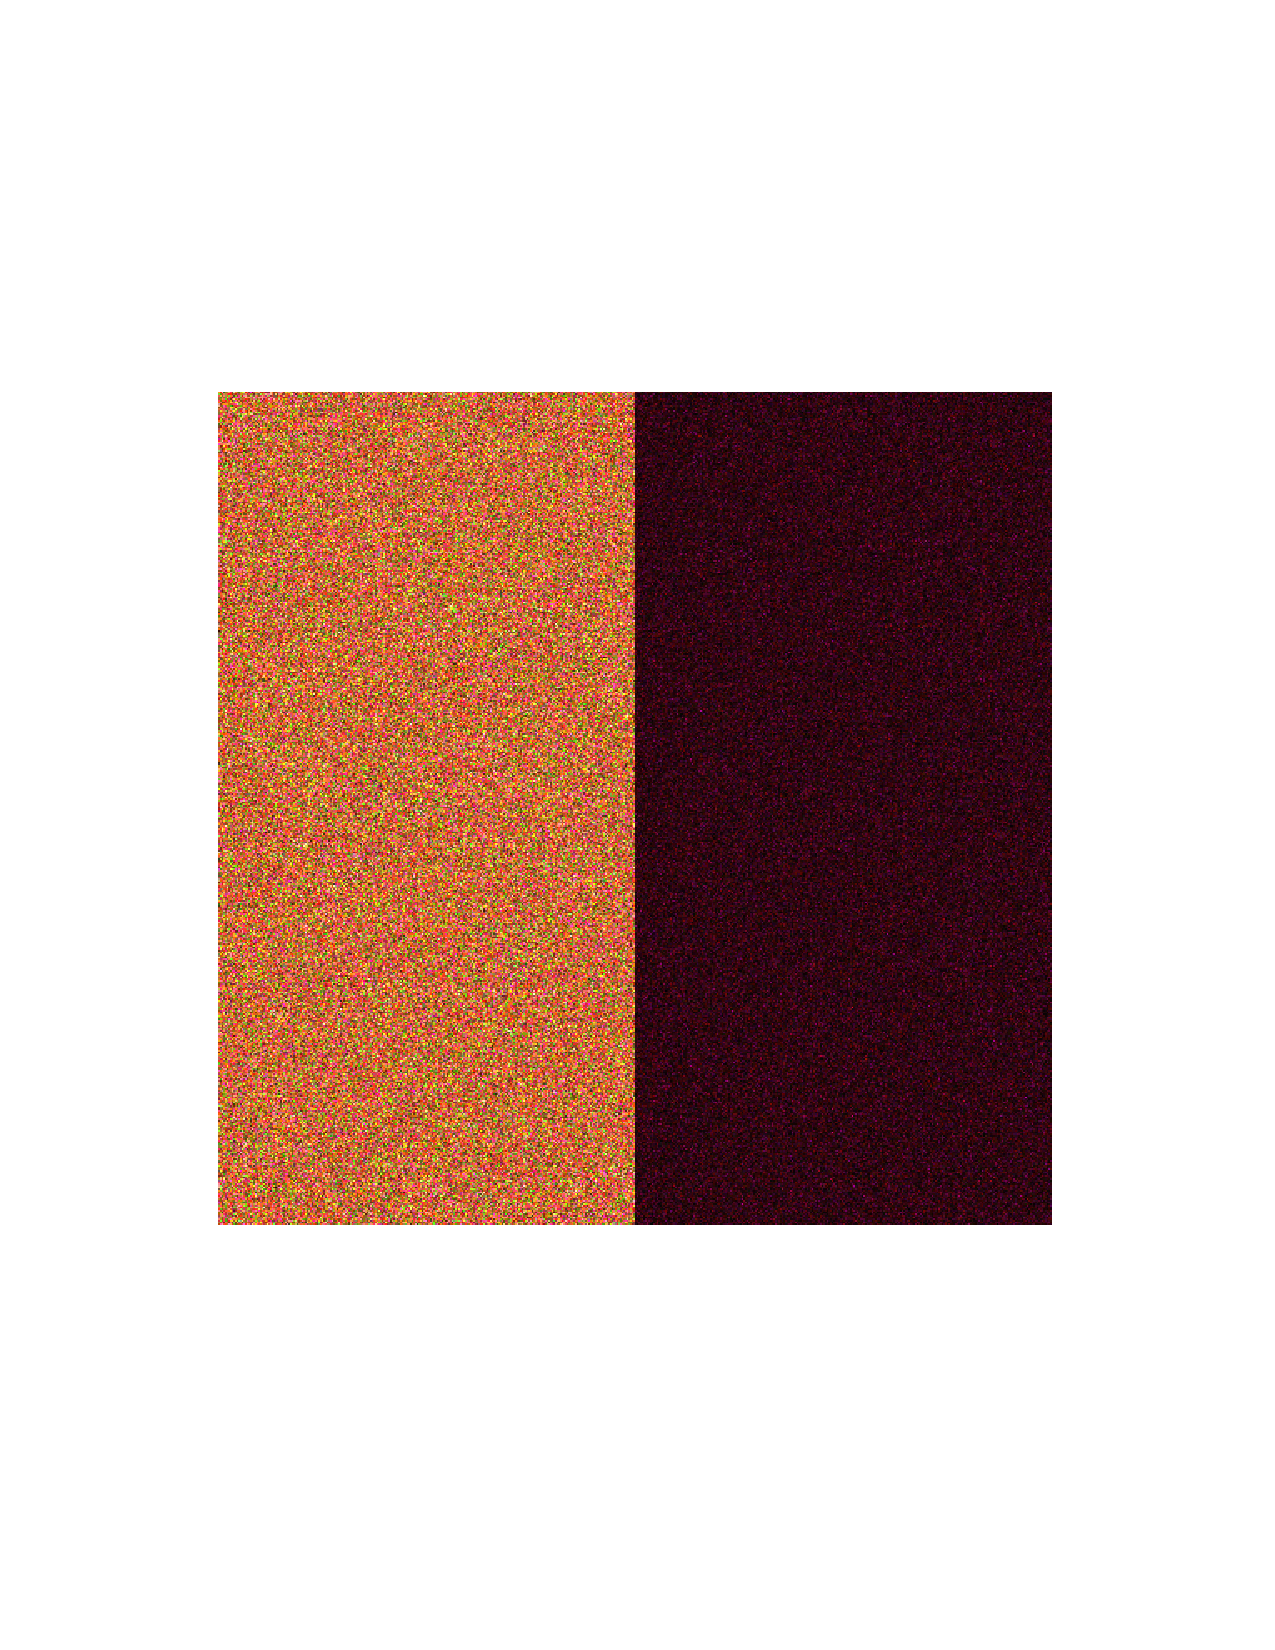
\includegraphics[width=.7\linewidth]{phanton_gamf_dec_pauli}%
	\caption{Pauli decomposition}
\label{simulada_gamf_dec_pauli}
\end{figure}


The Pauli decomposition is based on the linear combination of intensity channels: $(\mathbf{I_\text{hh}+I_{\text{vv}}}, \mathbf{I_\text{hh}-I_{\text{vv}}}, \mathbf{I_\text{hv}})$. This decomposition shows the evidence of edge in the middle line, as presented in Fig.~\ref{fig_Edges-Evidence}\subref{fig_Edges-Evidence:a}. 

Fig.~\ref{fig_Edges-Evidence}\subref{fig_Edges-Evidence:b}. 
shows the density function of $\sigma_\text{hh}$ with parameters extracted from real data for forest and urban areas: $\sigma_\text{hh}=962892$ and $\sigma_\text{hh}= 360932$.  
    
\begin{figure}[hbt]
	\centering
     \subfloat[Channel $\text{hh}$ \label{fig_evid_bordas:1a}]{%
       %\includegraphics[width=0.2\textwidth]{example-image-a}
       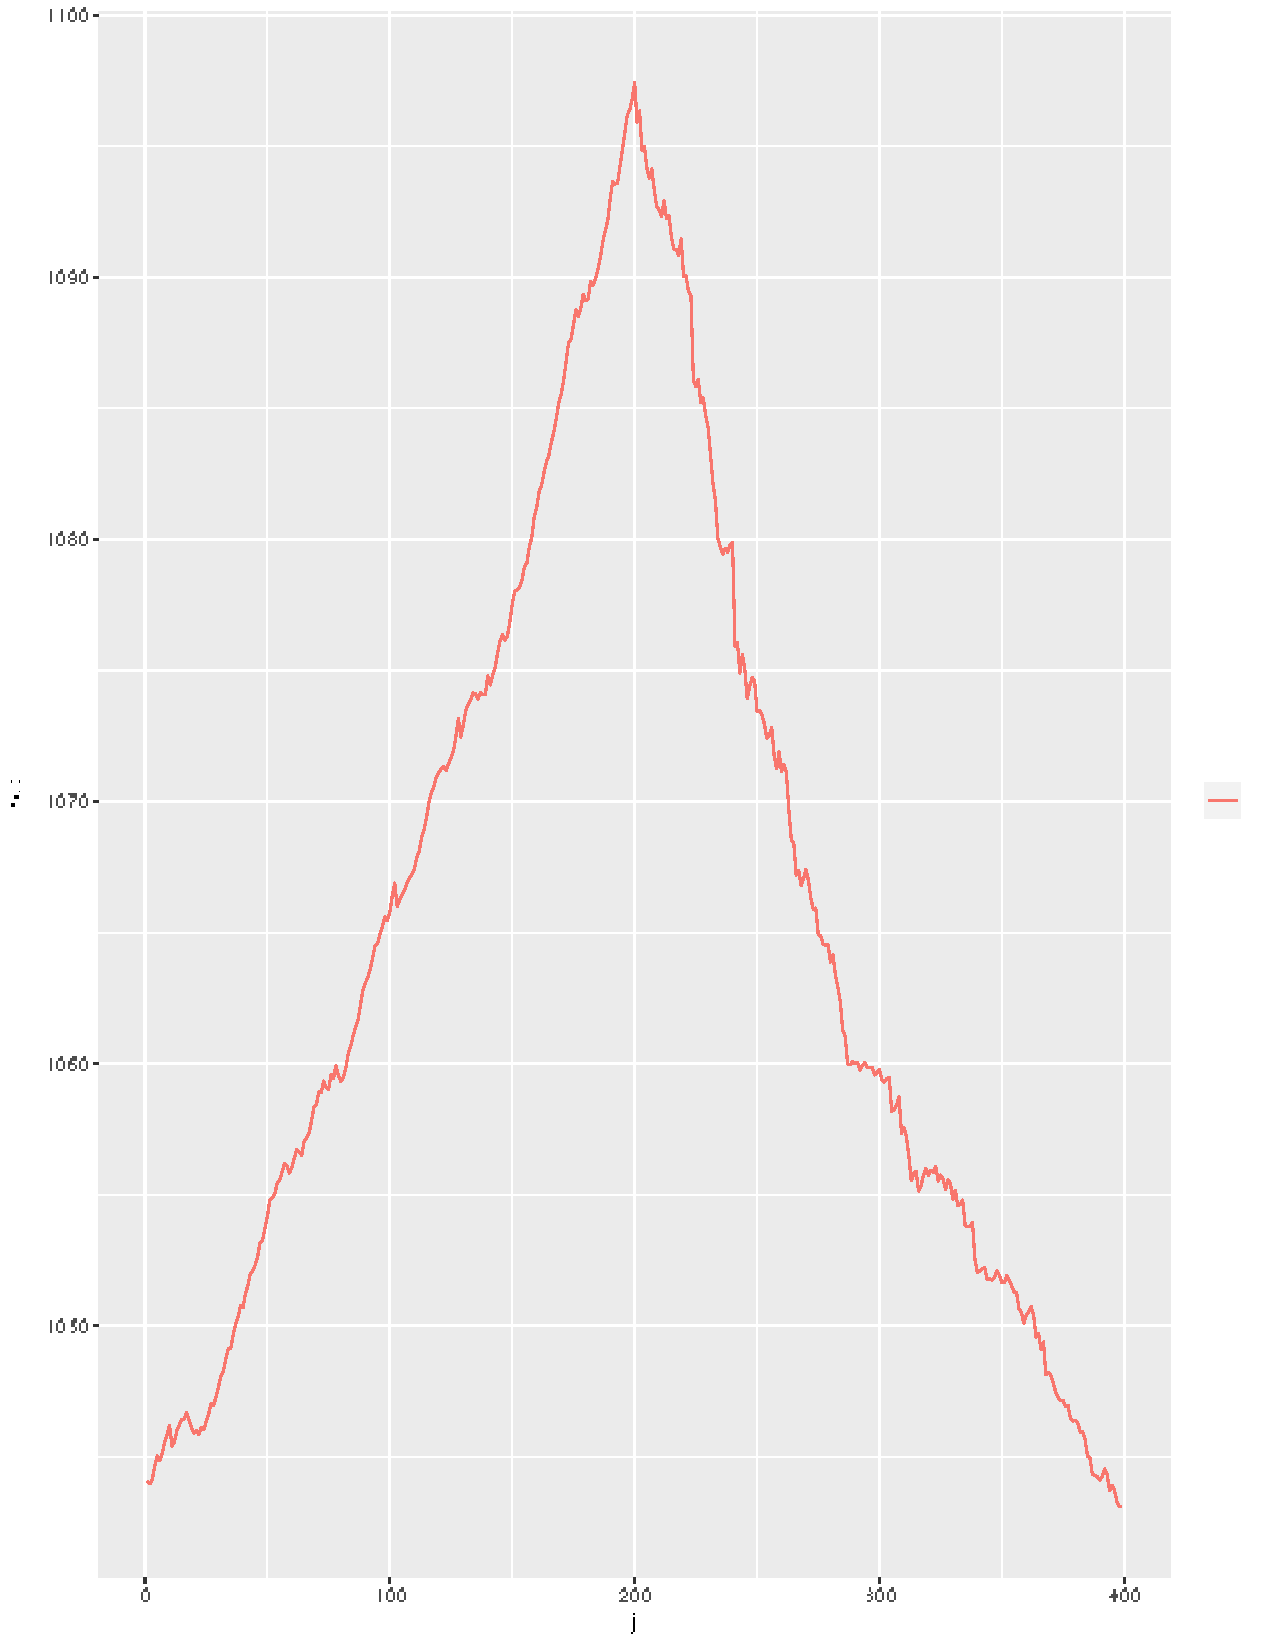
\includegraphics[width=0.32\linewidth]{grafico_l_gamf_2017_sigmahh_param_mu}}
     \subfloat[Channel $\text{hv}$ \label{fig_evid_bordas:1b}]{%
       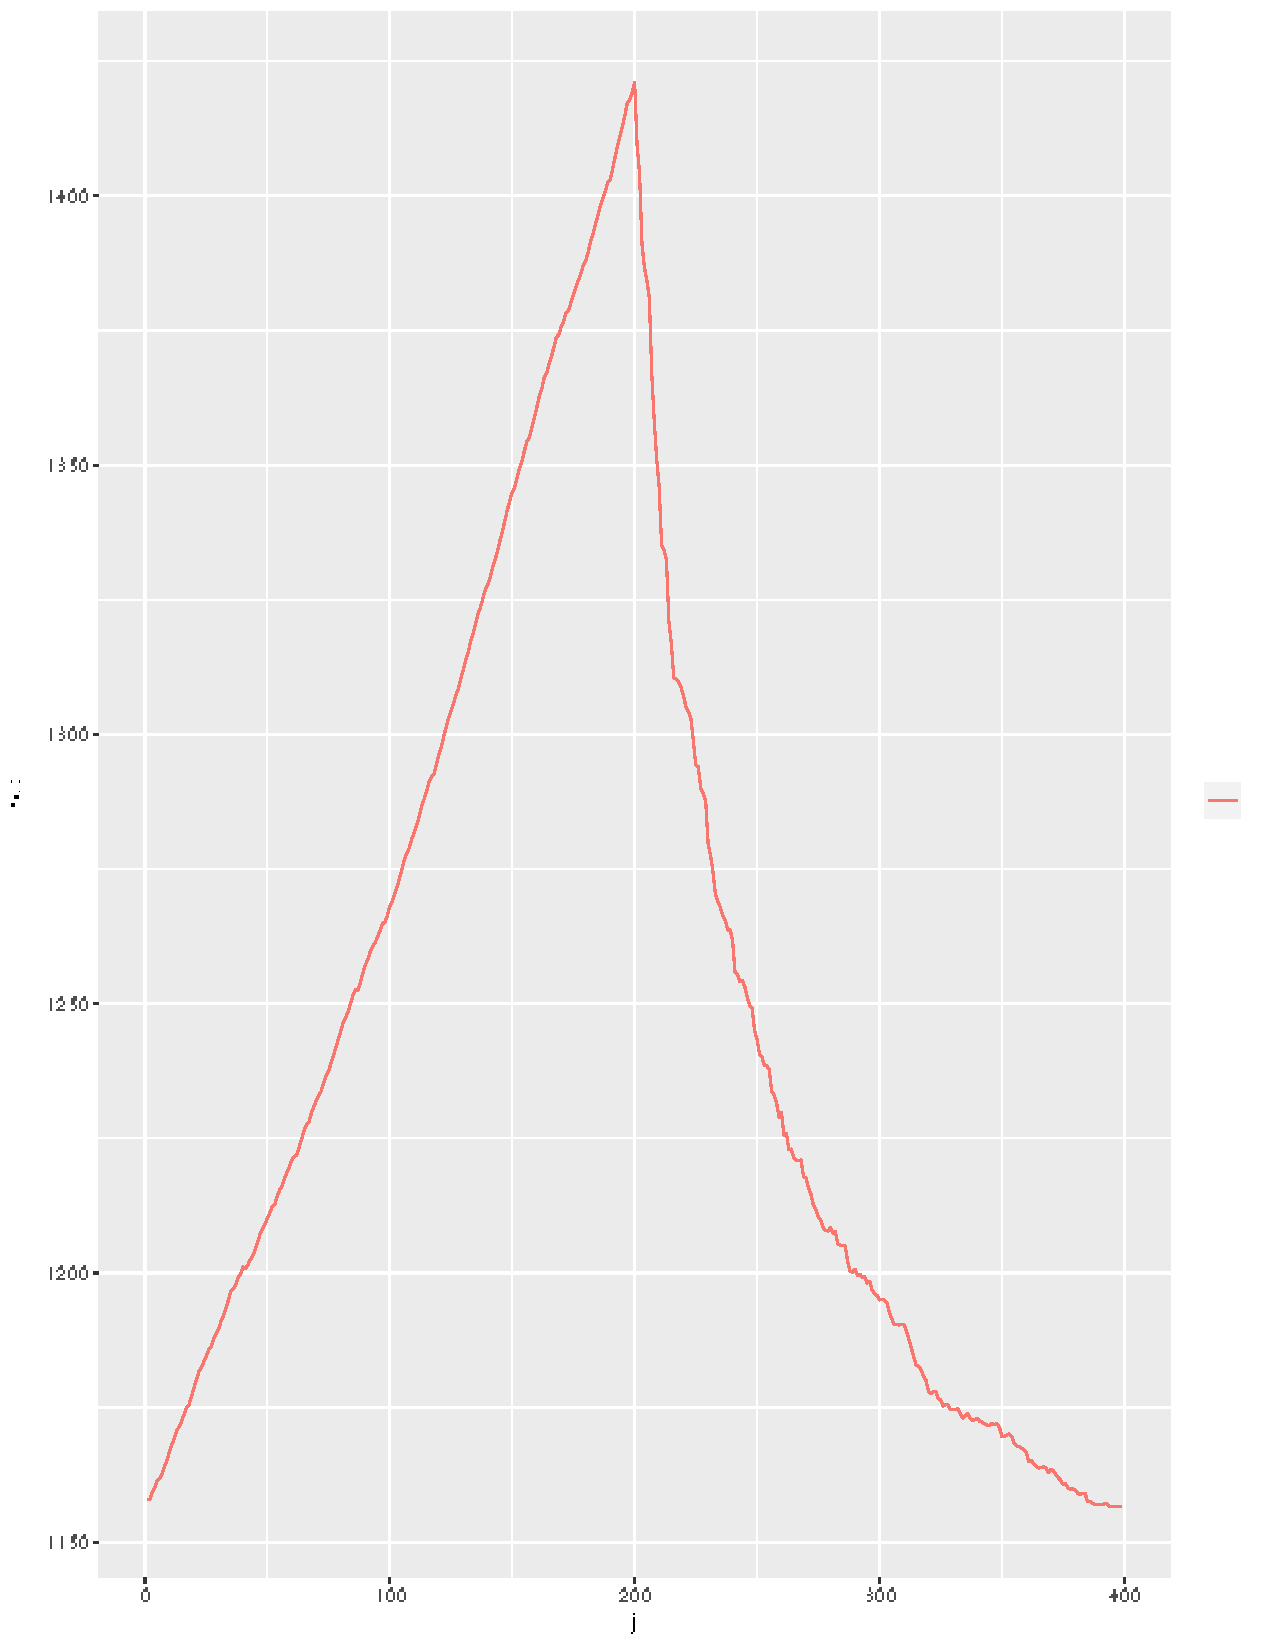
\includegraphics[width=0.32\linewidth]{grafico_l_gamf_2017_sigmahv_param_mu}}
     \subfloat[Channel $\text{vv}$ \label{fig_evid_bordas:1c}]{%
       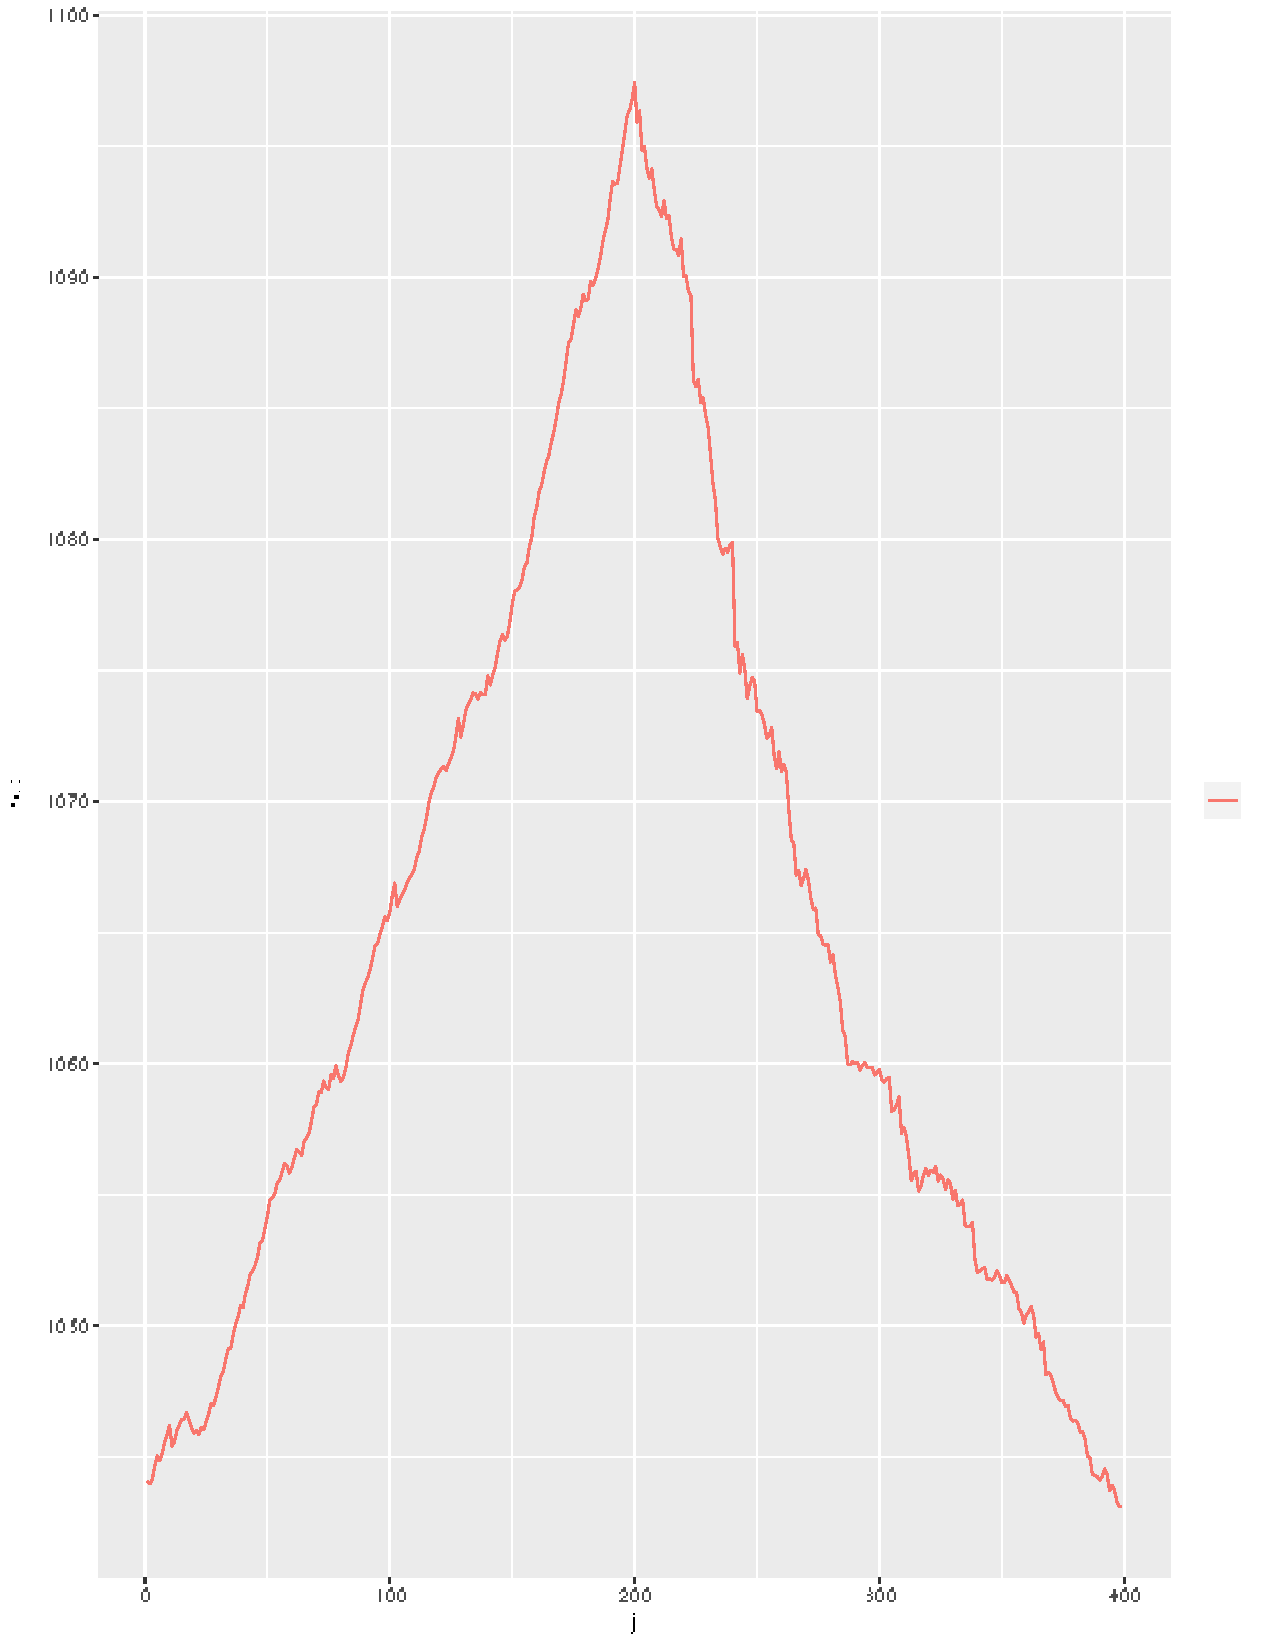
\includegraphics[width=0.32\linewidth]{grafico_l_gamf_2017_sigmahh_param_mu}}
     \caption{Edges evidences in one radial}
     \label{fig_evid_bordas}
   \end{figure}	





The functions have a peak indicating the evidence of the edge that should be captured, but the functions are not smooth, hindering the use of optimization methods that require the calculation of the derivative.
This problem was solved using Generalized Simulated Annealing (GenSA)~\cite{xgsh}, suitable for non-differentiable functions.
    
The error is measured simulating $400$ independent images and finding $\widehat\jmath$ in a line fixed.
By construction, the vertical line $200$ is considered as the real edge in each replication, so the error for this replication is the absolute value of the difference between this point and the estimated value, and it is computed by $E(r) = |200 - \widehat{\jmath}(r)|$, $1\leq r \leq 400$.

Relative frequencies to estimate the probability of having an error smaller than a number of pixels is used. 
Denoting $H(k)$ the number of replications for which the error is less than $k$ pixels, an estimate of this probability is $f(k)=\frac{H(k)}{400}$. 
In the tests performed in this section, $k$ varies between $1$ and $10$. 
The algorithm is described in Ref.~\cite{fbgm}.
Fig.~\ref{probability_edge_detc} shows these probabilities as computed in each channel $I_\text{hh}$, $I_\text{hv}$ and $I_{vv}$ of the image. 
  
%\begin{figure}[hbt]
%	\centering
%	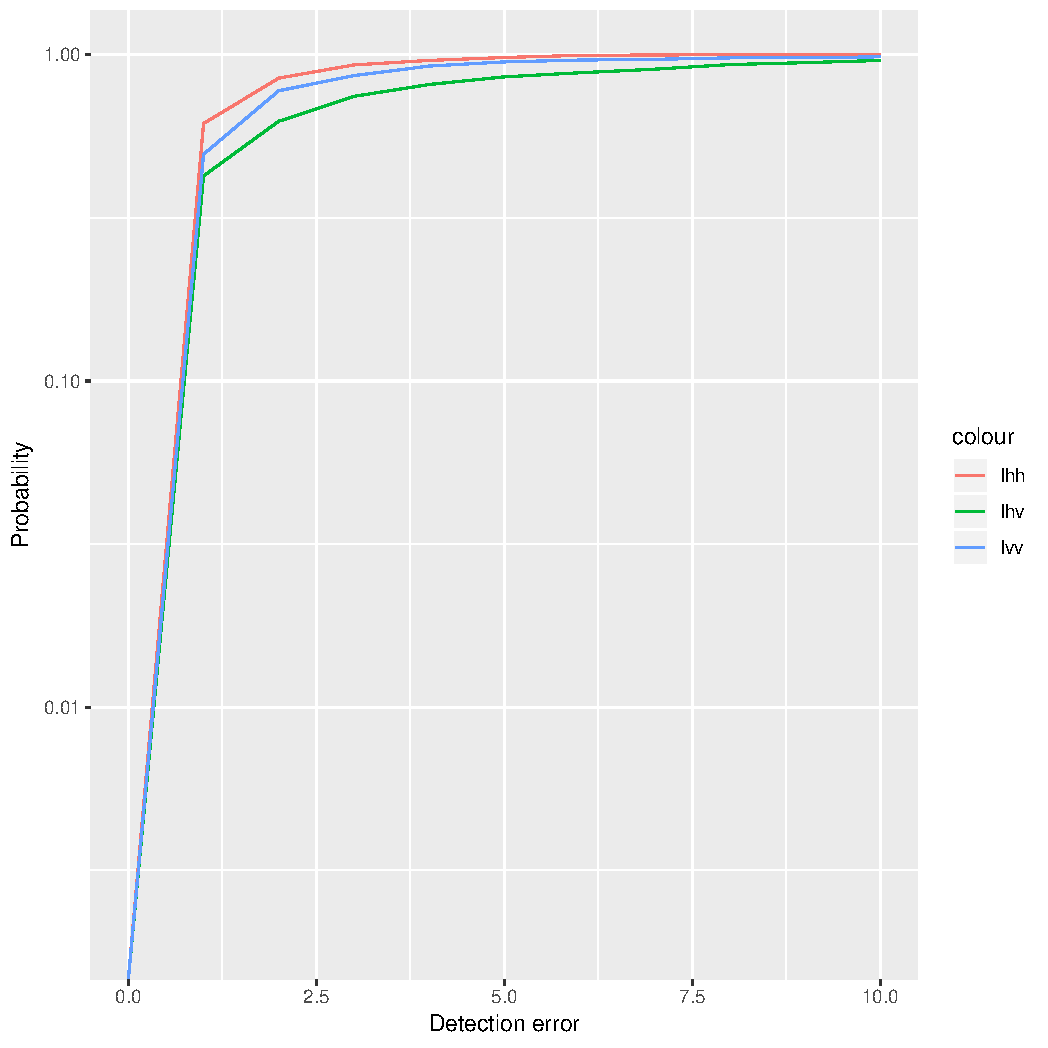
\includegraphics[width=.7\linewidth]{metricas_ihh_ivh_ivv_nhfc_artigos}%
%	\caption{Probability of detecting edges evidences.}
%\label{probability_edge_detc}
%\end{figure}

   \begin{figure*}[hbt]
	\centering
     \subfloat[Evidences in channel $\text{hh}$ \label{evidencias_hh_hv_vv:a}]{%
       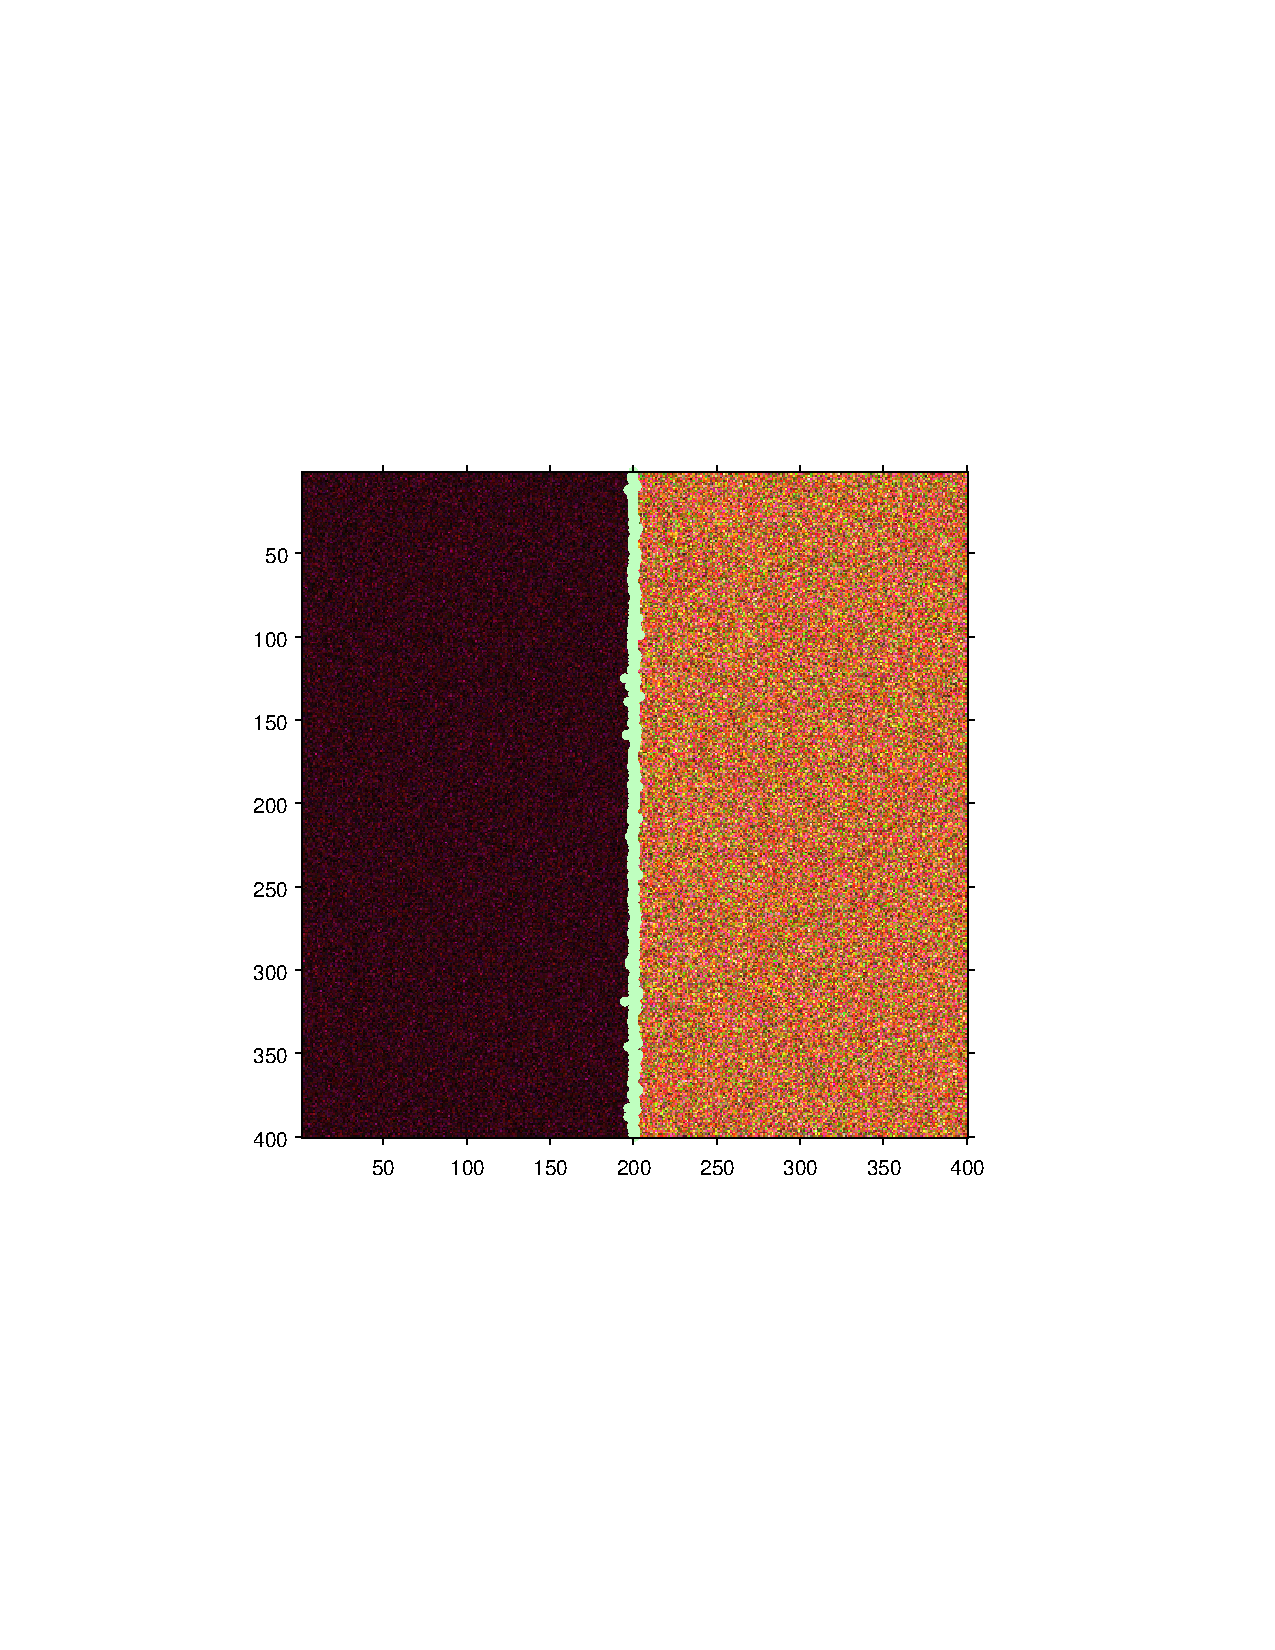
\includegraphics[width=0.35\linewidth]{im_sim_gamf_hh_evid_param_mu_14_pixel}
     }
     \subfloat[Evidences in channel $\text{hv}$ \label{evidencias_hh_hv_vv:b}]{%
       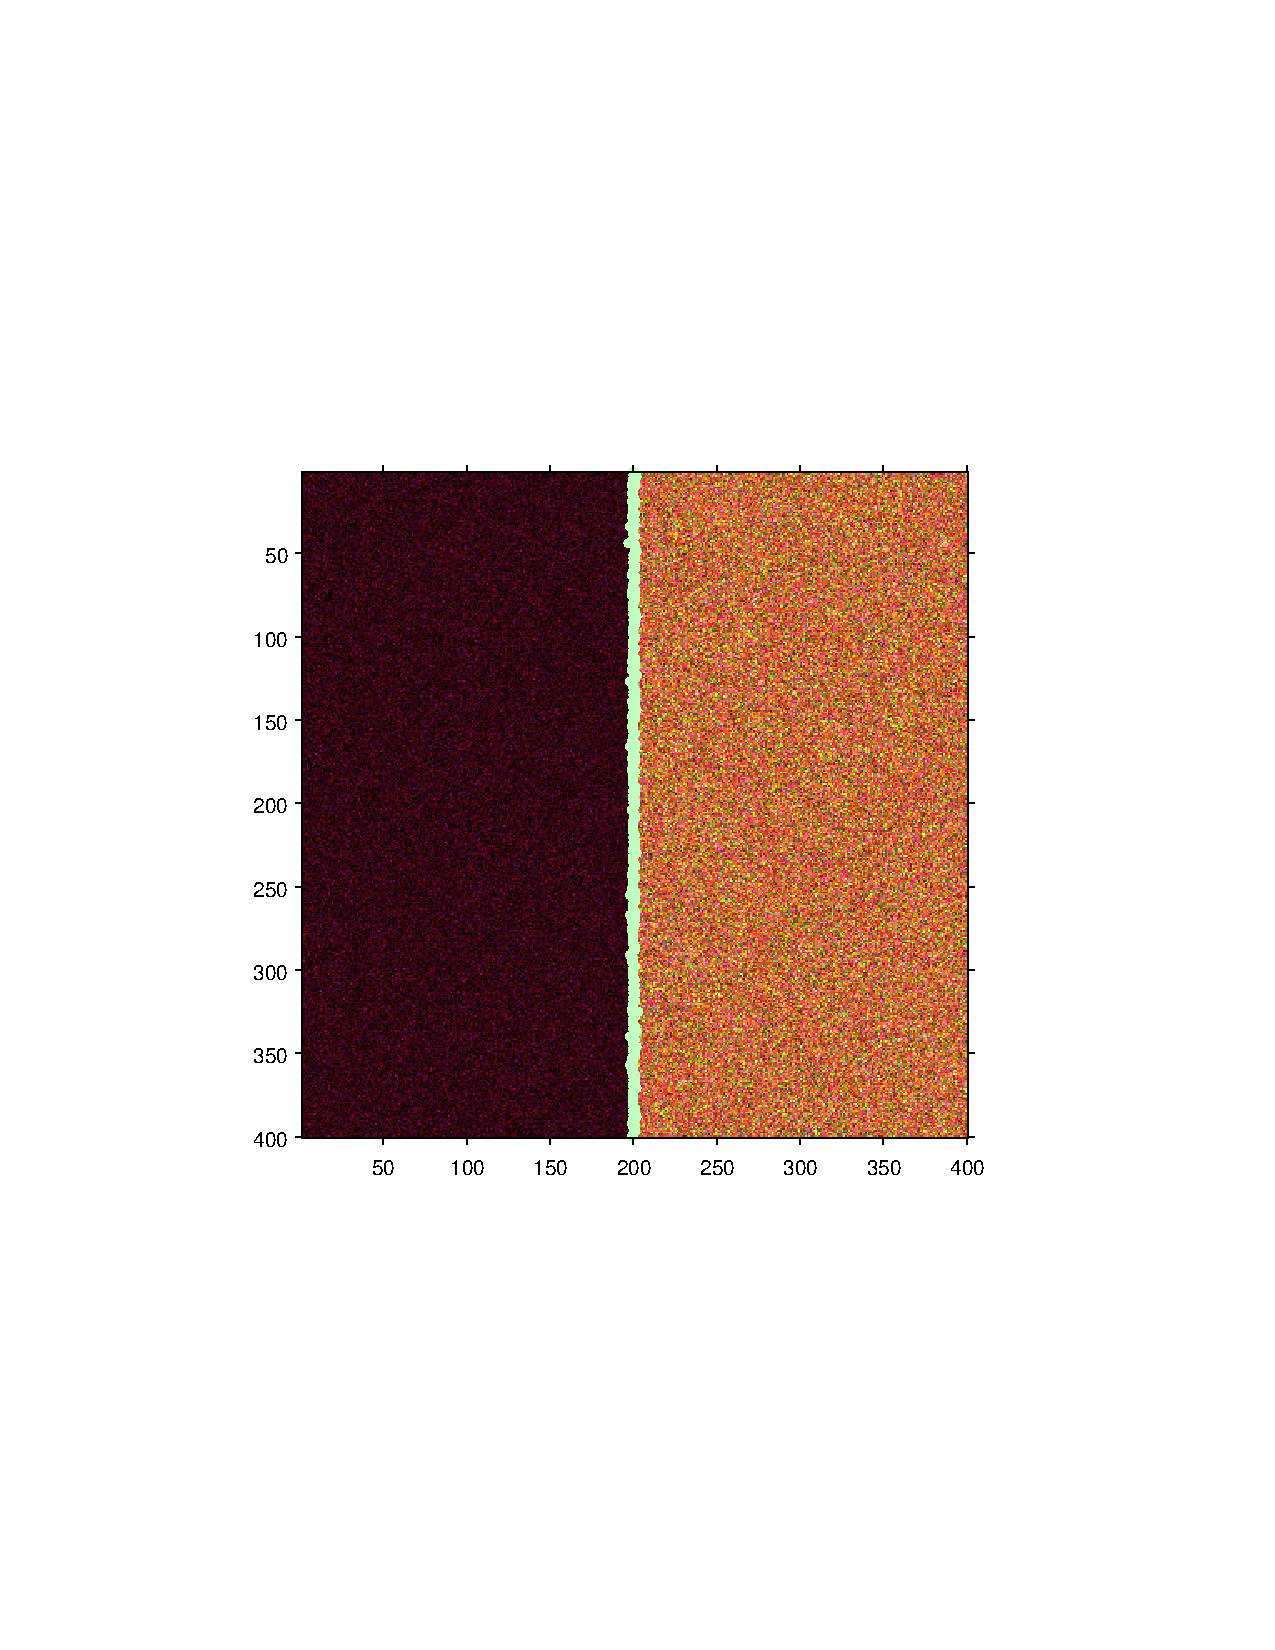
\includegraphics[width=0.35\linewidth]{im_sim_gamf_hv_evid_param_mu_14_pixel}
     }
     \subfloat[Evidences in channel $\text{vv}$ \label{evidencias_hh_hv_vv:c}]{%
       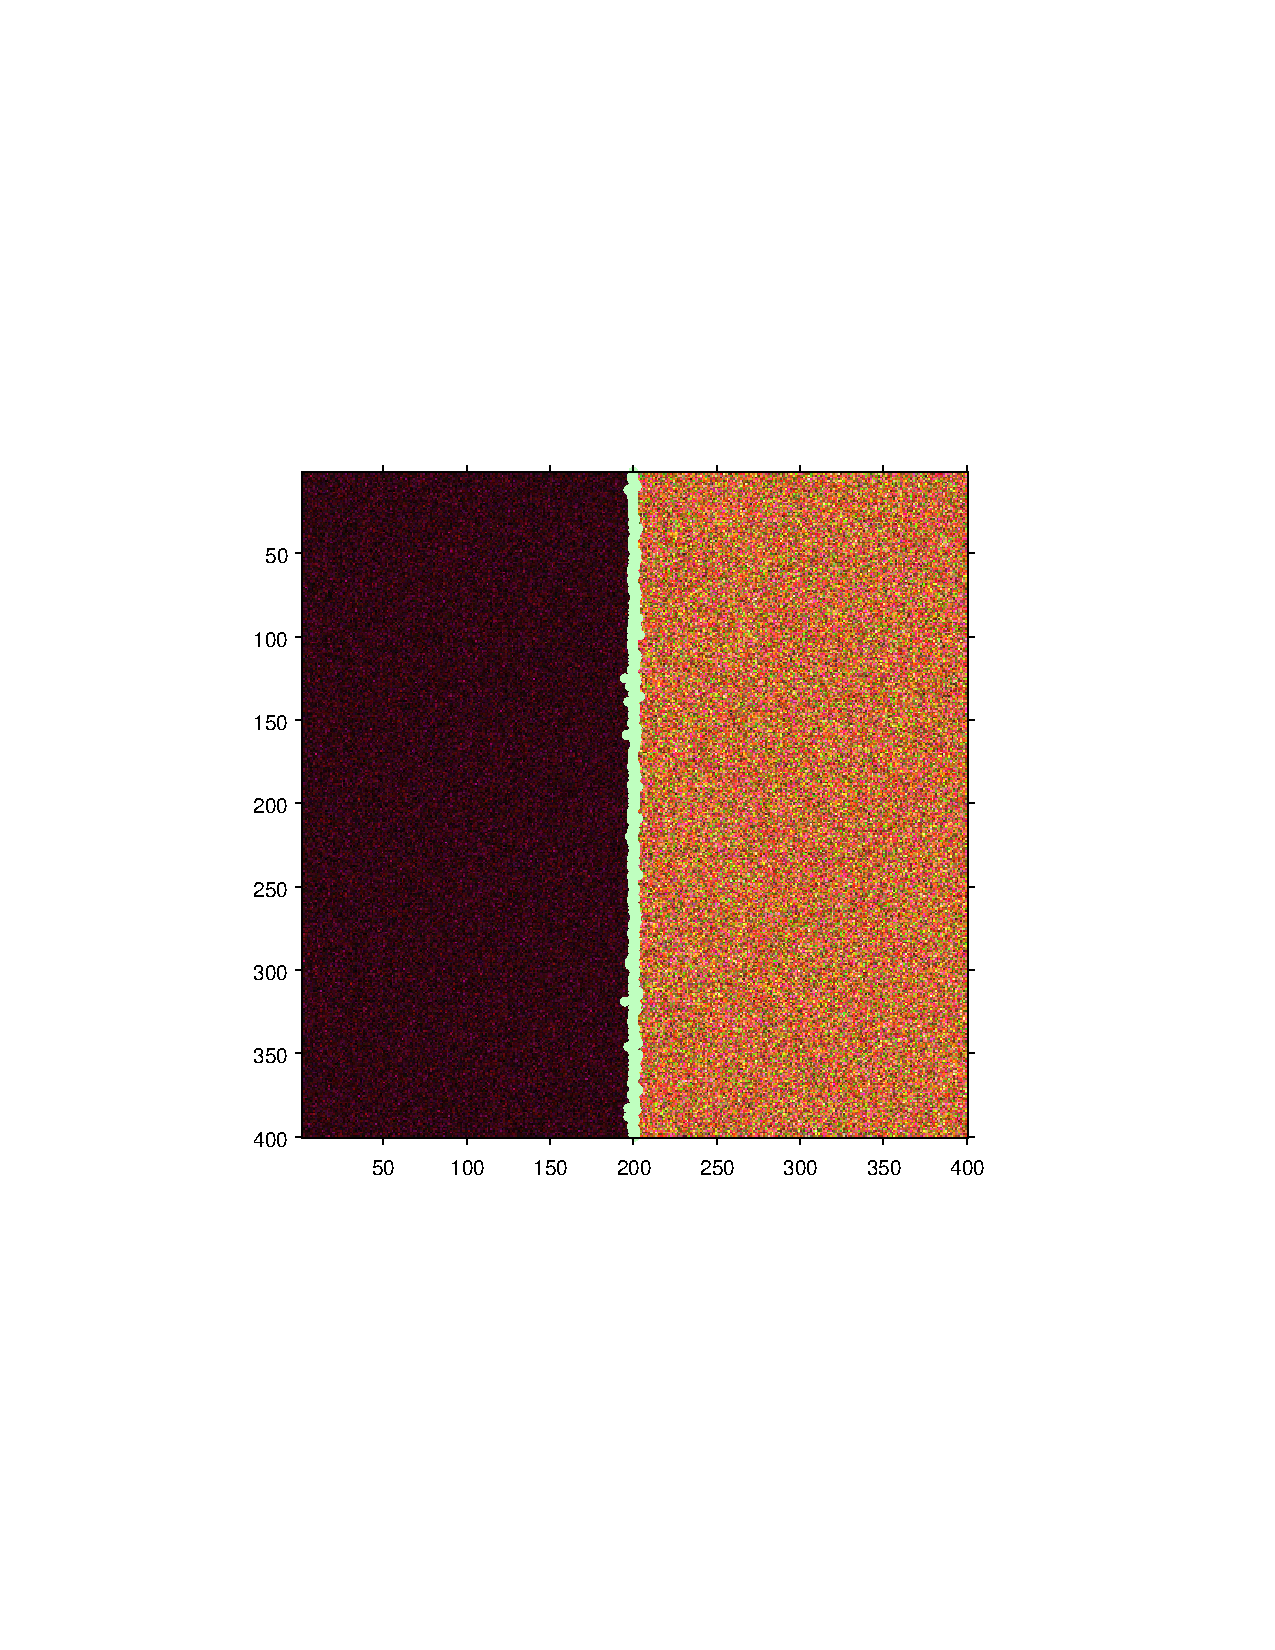
\includegraphics[width=0.35\linewidth]{im_sim_gamf_vv_evid_param_mu_14_pixel}
     }
     \caption{Edges evidences from the three intensity channels to estimated $\mu$}
     \label{evidencias_hh_hv_vv} 
   \end{figure*}
   
   
   \begin{figure*}[hbt]
	\centering
     \subfloat[Evidences in channel $\text{hh}$ \label{evidencias_hh_hv_vv:a}]{%
       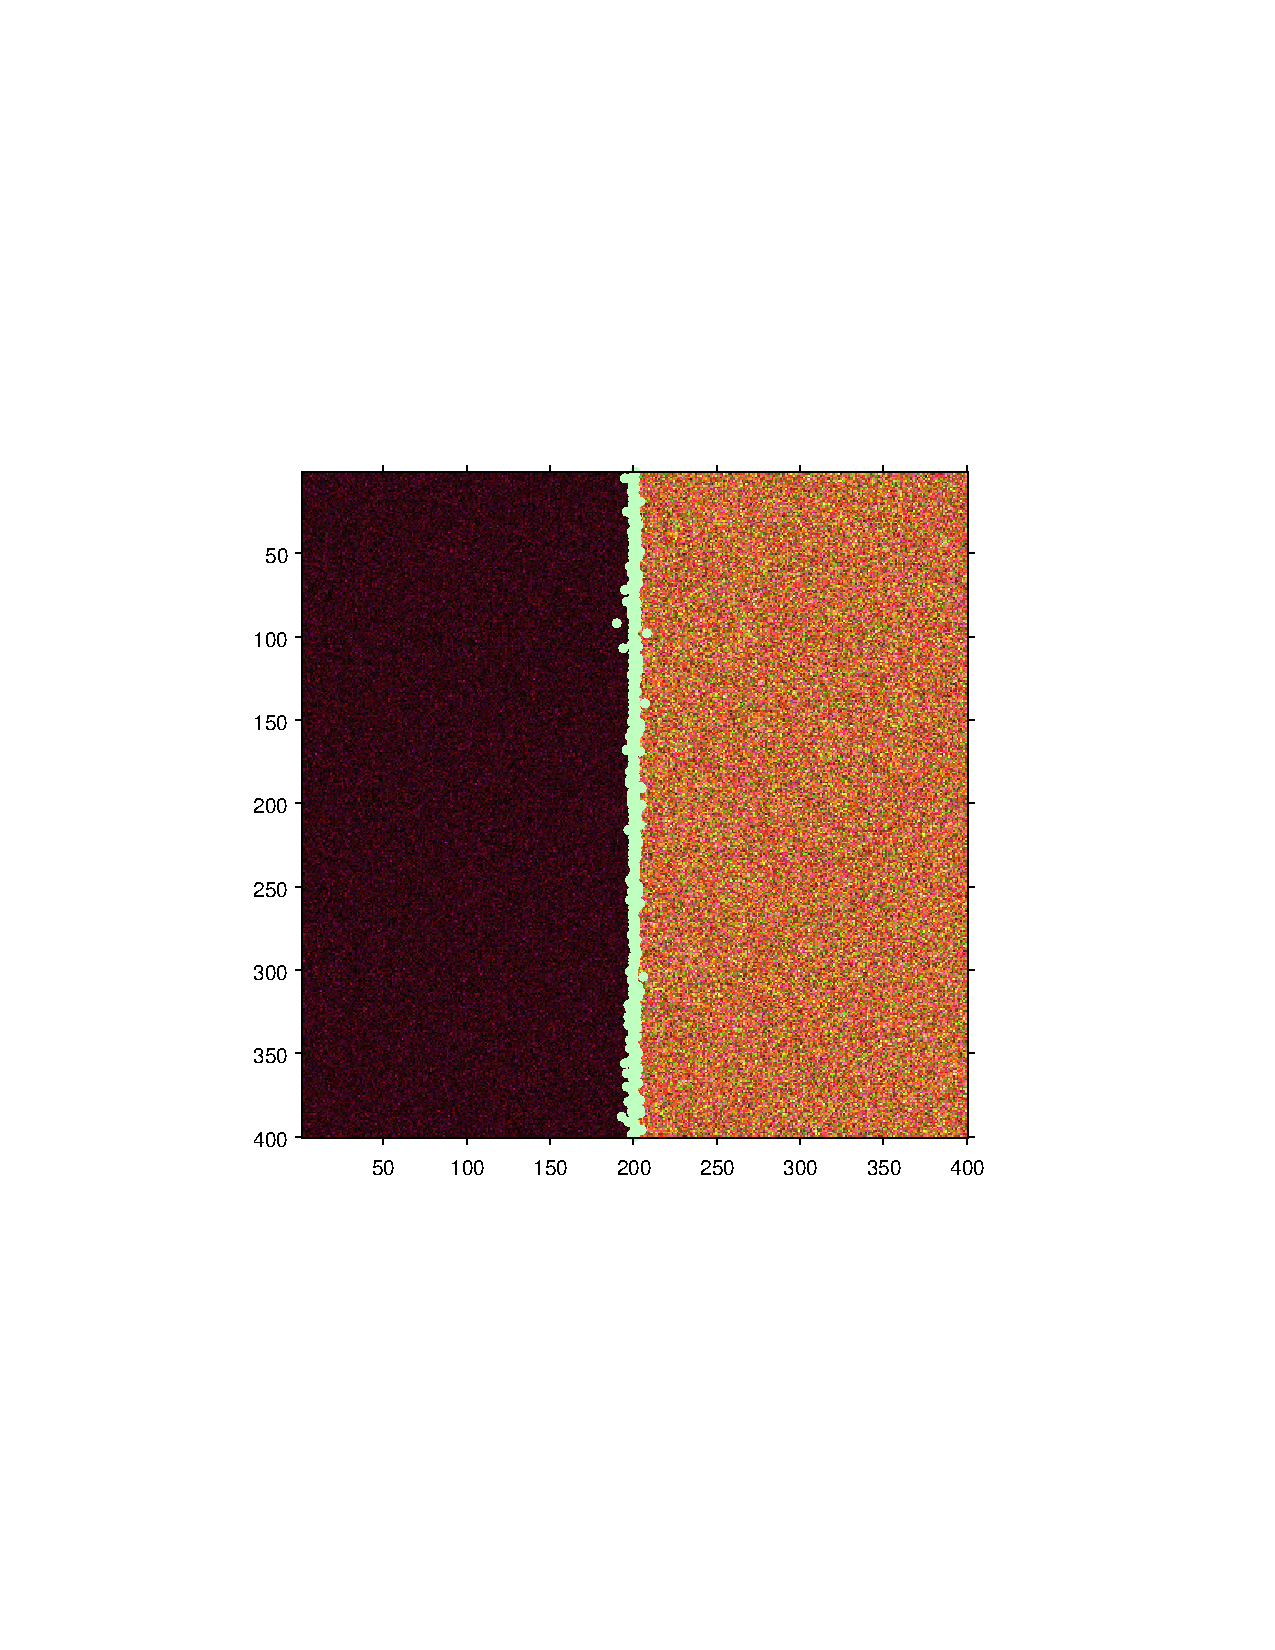
\includegraphics[width=0.35\linewidth]{im_sim_gamf_hh_evid_media_mu_14_pixel}
     }
     \subfloat[Evidences in channel $\text{hv}$ \label{evidencias_hh_hv_vv:b}]{%
       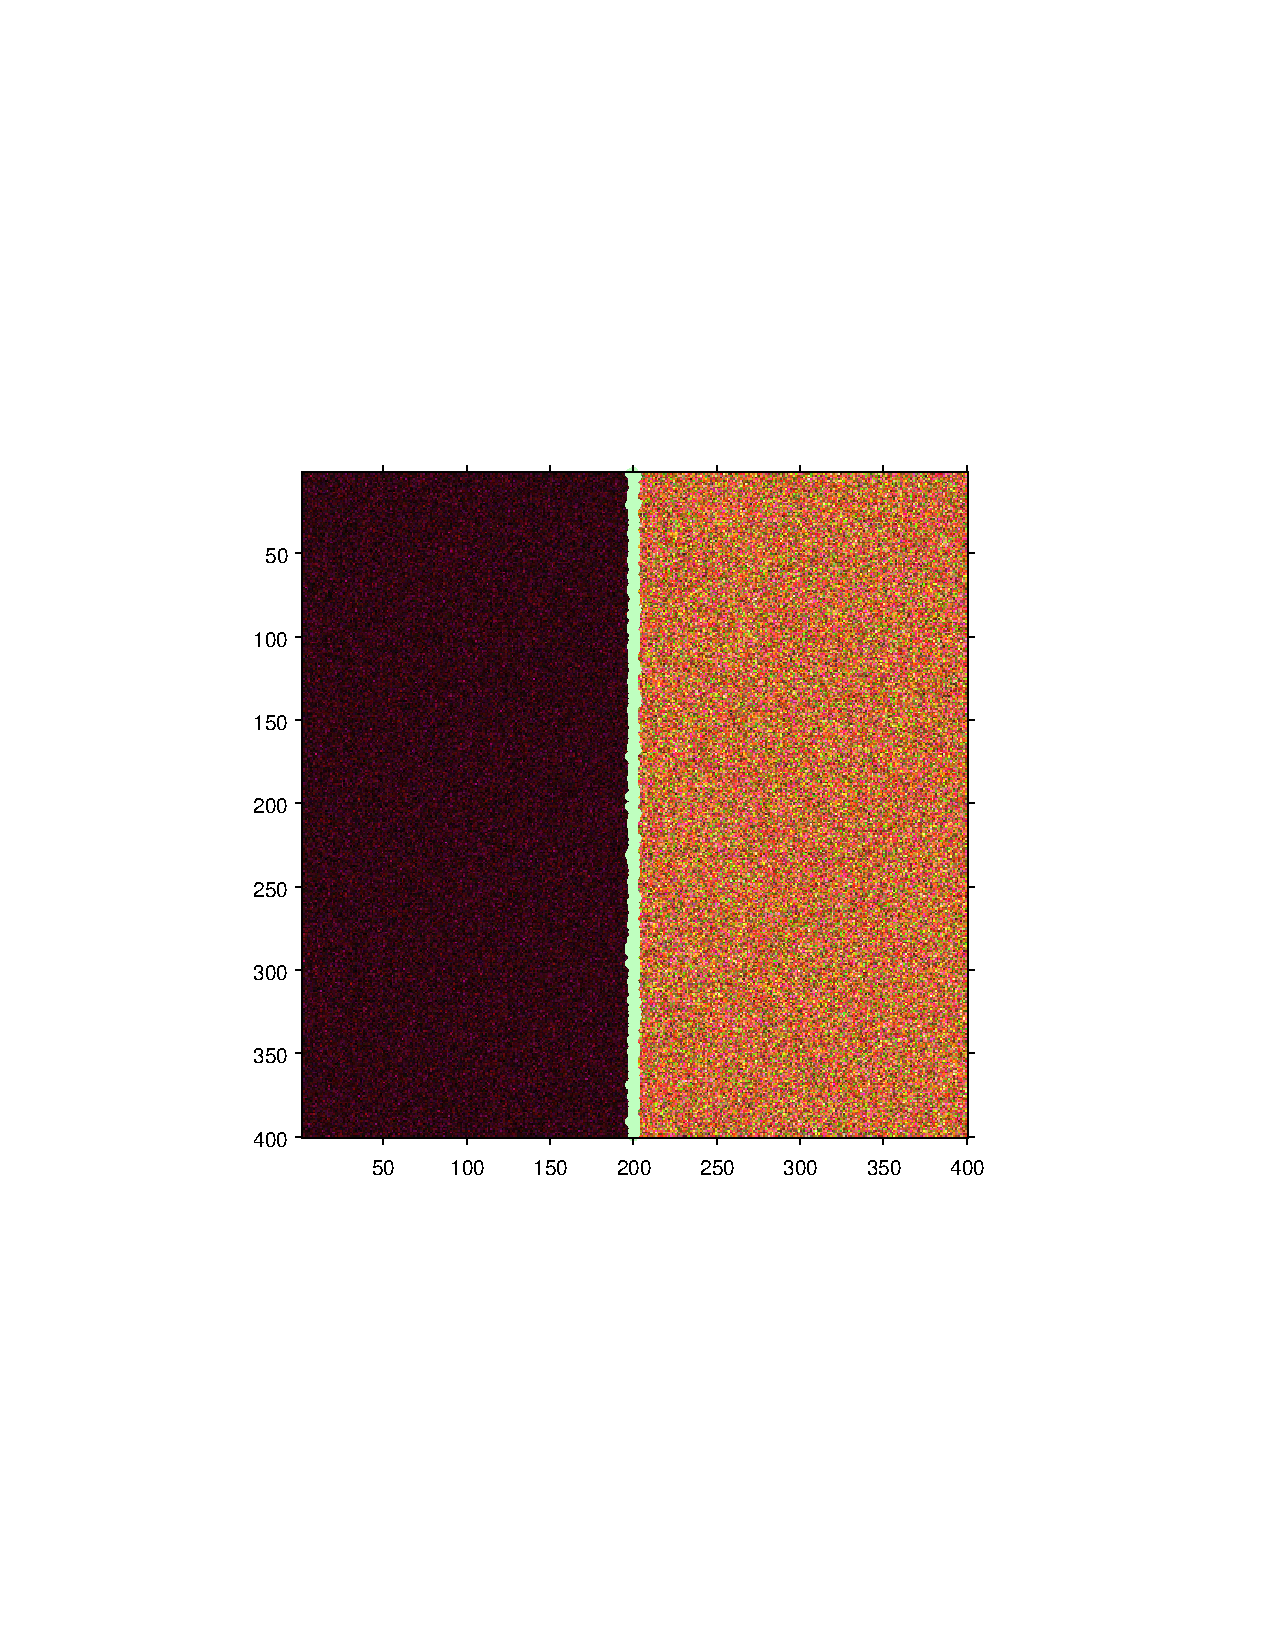
\includegraphics[width=0.35\linewidth]{im_sim_gamf_hv_evid_media_mu_14_pixel}
     }
     \subfloat[Evidences in channel $\text{vv}$ \label{evidencias_hh_hv_vv:c}]{%
       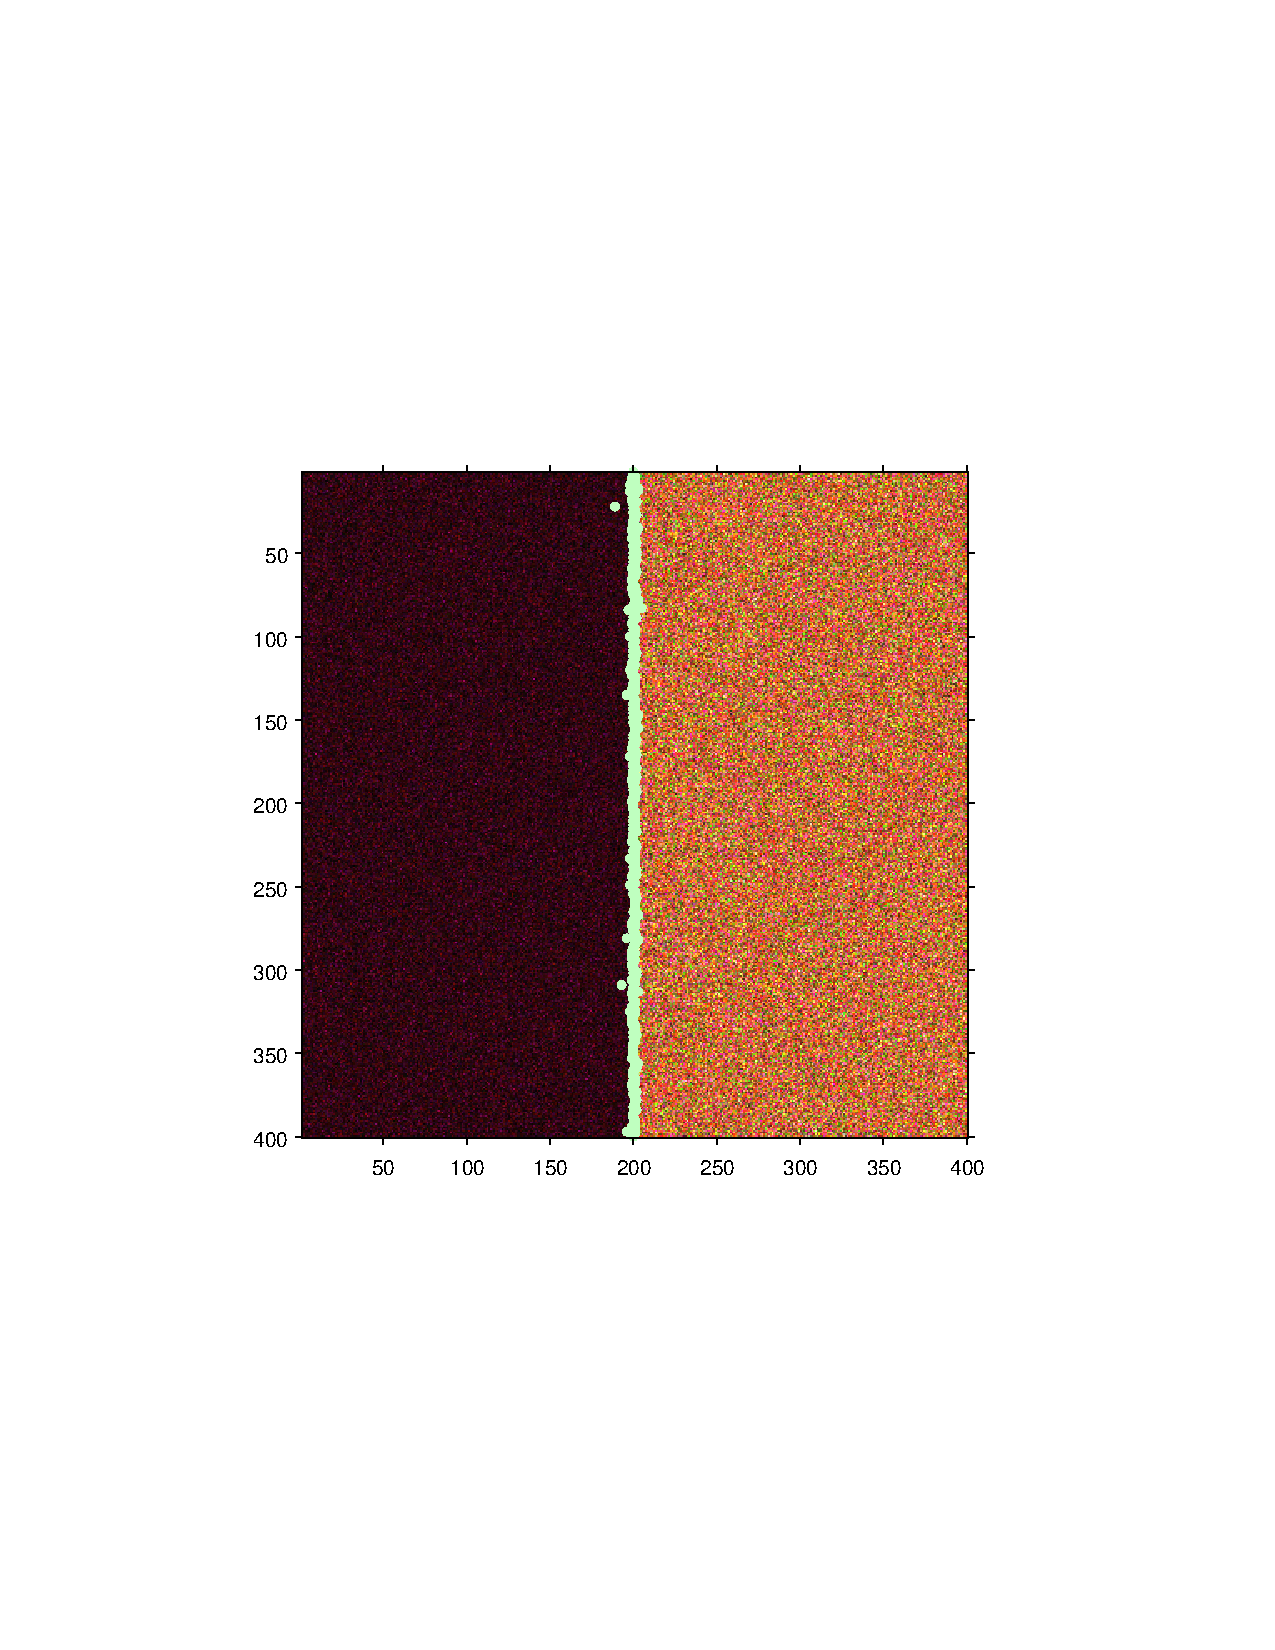
\includegraphics[width=0.35\linewidth]{im_sim_gamf_vv_evid_media_mu_14_pixel}
     }
     \caption{Edges evidences from the three intensity channels to estimated (media) $\mu$}
     \label{evidencias_hh_hv_vv} 
   \end{figure*}   
   
   
   
   
\subsubsection{Distribution univariate the product of intensity to several L fixed}



\begin{figure}[hbt]
	\centering
     \subfloat[Function $\ell$ from pixels 1 to 150 \label{fig:evid_bordas_l:1a}]{%
       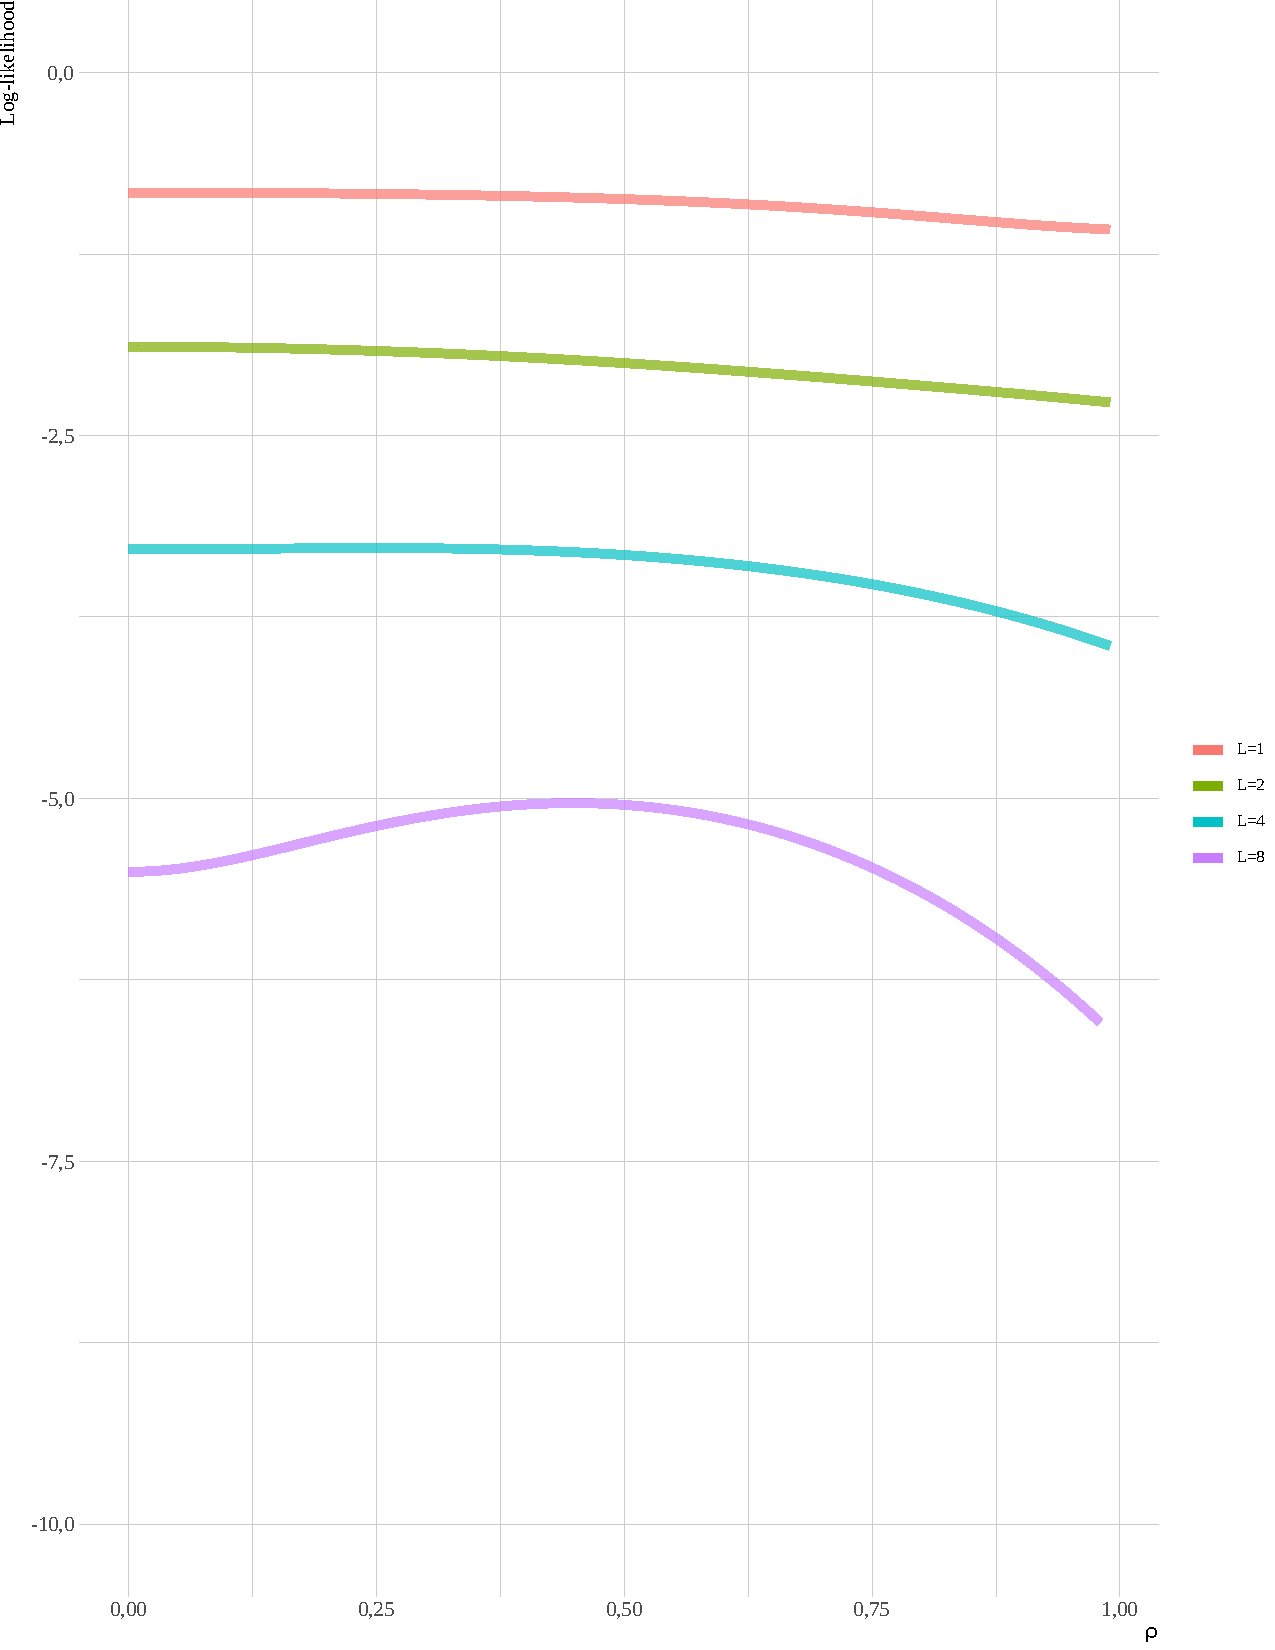
\includegraphics[width=0.32\linewidth]{log_like_prod_mag_L_fixo_ing}}
     \subfloat[Function $\ell$ from Pixels 150 to 400 \label{fig:evid_bordas_l:1b}]{%
       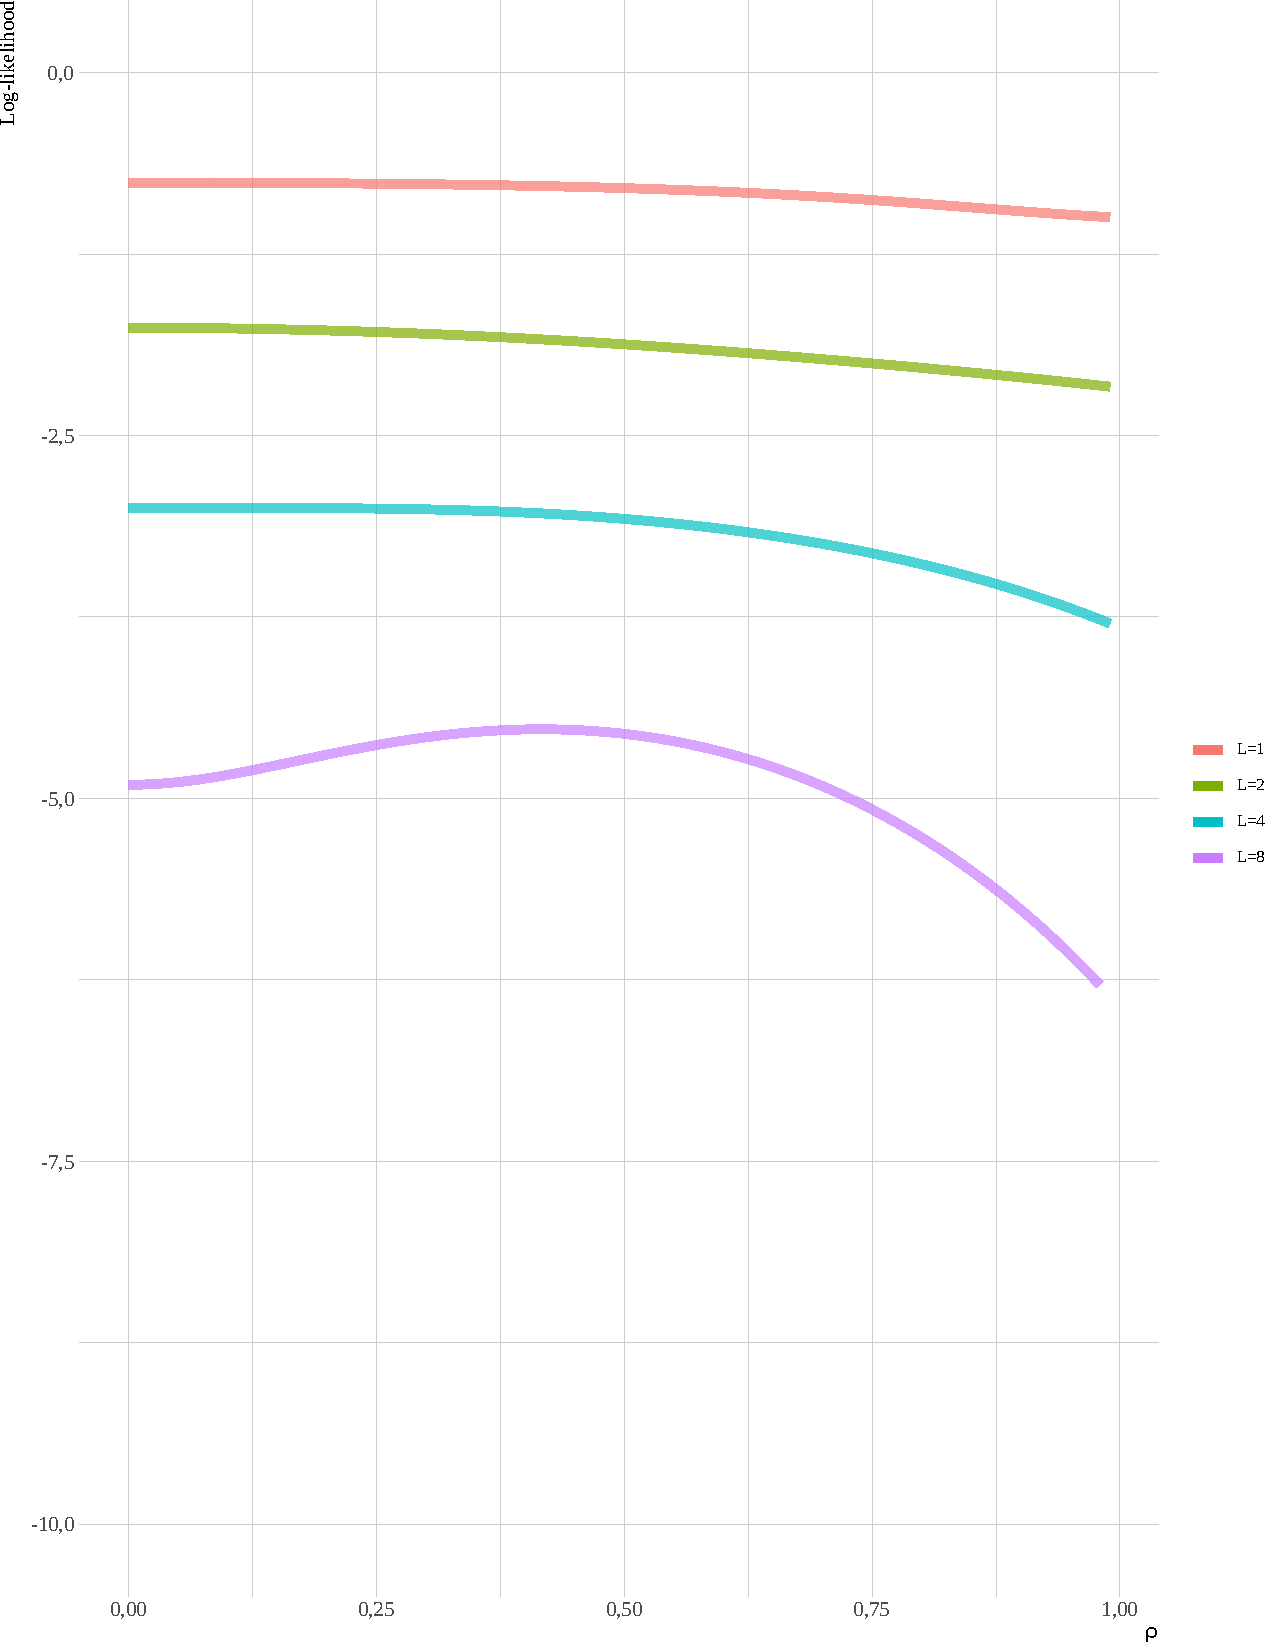
\includegraphics[width=0.32\linewidth]{log_like_prod_mag_L_fixo_ing_150_to_400}}
     %\subfloat[Canal $\text{vv}$ \label{fig:evid_bordas_l:1c}]{%
     %  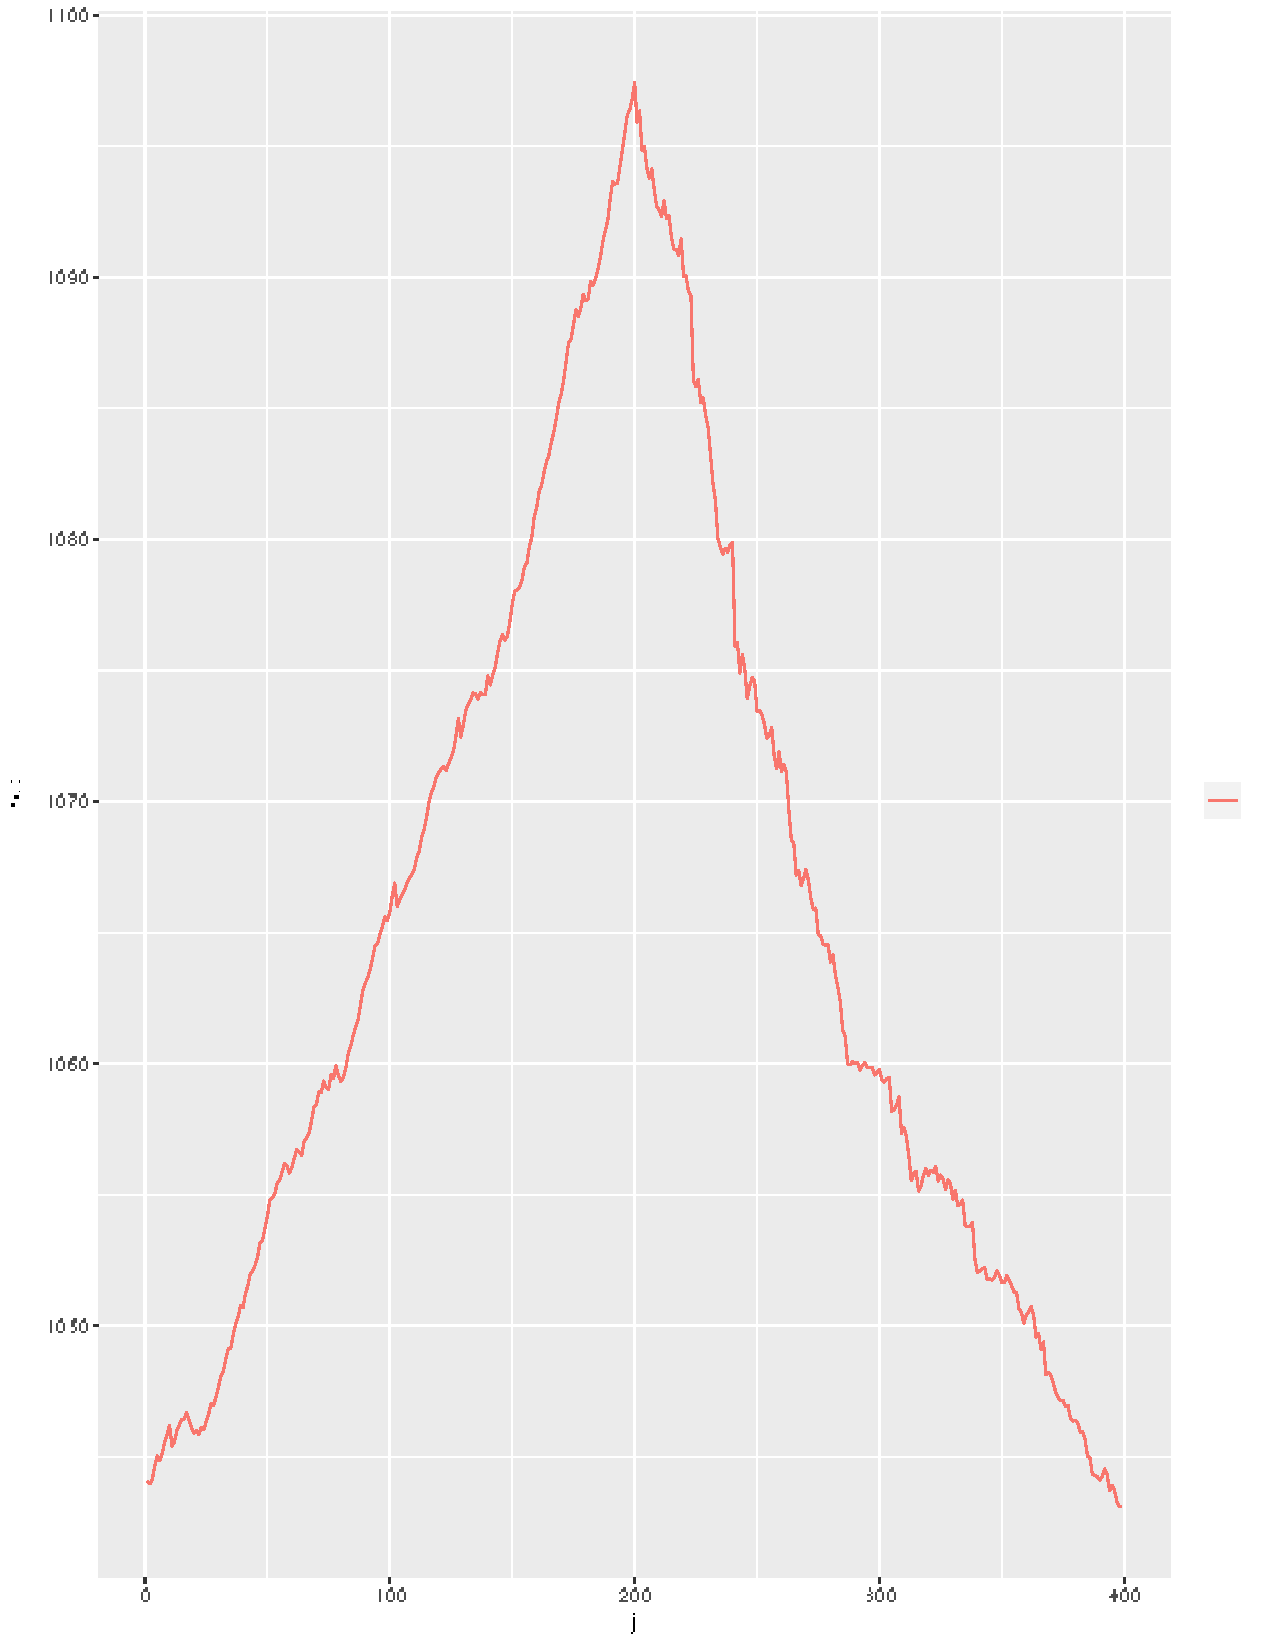
\includegraphics[width=0.32\linewidth]{grafico_l_gamf_2017_sigmahh_param_mu}}
     \caption{Distribution product of intensities to several L fixed and radial equal 35}
     \label{fig:evid_bordas_l}
   \end{figure}	

\subsection{Application to Actual Data}
\section{Discussion}


%This section may be divided by subheadings. It should provide a concise and precise description of the experimental results, their interpretation as well as the experimental conclusions that can be drawn.
\begin{quote}
This section may be divided by subheadings. It should provide a concise and precise description of the experimental results, their interpretation as well as the experimental conclusions that can be drawn.
\end{quote}

%%%%%%%%%%%%%%%%%%%%%\begin{equation}
%\end{equation}%%%%%%%%%%%%%%%%%%%%%
%\subsection{Subsection}
%\unskip
%\subsubsection{Subsubsection}

%Bulleted lists look like this:
%\begin{itemize}[leftmargin=*,labelsep=5.8mm]
%\item	First bullet
%\item	Second bullet
%\item	Third bullet
%\end{itemize}

%Numbered lists can be added as follows:
%\begin{enumerate}[leftmargin=*,labelsep=4.9mm]
%\item	First item 
%\item	Second item
%\item	Third item
%\end{enumerate}

%The text continues here.

%\subsection{Figures, Tables and Schemes}

%All figures and tables should be cited in the main text as Figure 1, Table 1, etc.

%\begin{figure}[H]
%\centering
%
\includegraphics[width=2 cm]{Definitions/logo-mdpi}
%\caption{This is a figure, Schemes follow the same formatting. If there are multiple panels, they should be listed as: (\textbf{a}) Description of what is contained in the first panel. (\textbf{b}) Description of what is contained in the second panel. Figures should be placed in the main text near to the first time they are cited. A caption on a single line should be centered.}
%\end{figure}   
 
%Text

%Text

%\begin{table}[H]
%\caption{This is a table caption. Tables should be placed in the main text near to the first time they are cited.}
%\centering
%% \tablesize{} %% You can specify the fontsize here, e.g., \tablesize{\footnotesize}. If commented out \small will be used.
%\begin{tabular}{ccc}
%\toprule
%\textbf{Title 1}	& \textbf{Title 2}	& \textbf{Title 3}\\
%\midrule
%entry 1		& data			& data\\
%entry 2		& data			& data\\
%\bottomrule
%\end{tabular}
%\end{table}

%Text

%Text

%\begin{listing}[H]
%\caption{Title of the listing}
%\rule{\textwidth}{1pt}
%\raggedright Text of the listing. In font size footnotesize, small, or normalsize. Preferred format: left aligned and single spaced. Preferred border format: top border line and bottom border line.
%\rule{\textwidth}{1pt}
%\end{listing}


%\subsection{Formatting of Mathematical Components}

%This is an example of an equation:

%\begin{equation}
%a + b = c
%\end{equation}
%% If the documentclass option "submit" is chosen, please insert a blank line before and after any math environment (equation and eqnarray environments). This ensures correct linenumbering. The blank line should be removed when the documentclass option is changed to "accept" because the text following an equation should not be a new paragraph. 

%Please punctuate equations as regular text. Theorem-type environments (including propositions, lemmas, corollaries etc.) can be formatted as follows:
%% Example of a theorem:
%\begin{Theorem}
%Example text of a theorem.
%\end{Theorem}

%The text continues here. Proofs must be formatted as follows:

%% Example of a proof:
%\begin{proof}[Proof of Theorem 1]
%Text of the proof. Note that the phrase `of Theorem 1' is optional if it is clear which theorem is being referred to.
%\end{proof}
%The text continues here.

%%%%%%%%%%%%%%%%%%%%%%%%%%%%%%%%%%%%%%%%%%
%\section{Discussion}

%Authors should discuss the results and how they can be interpreted in perspective of previous studies and of the working hypotheses. The findings and their implications should be discussed in the broadest context possible. Future research directions may also be highlighted.

%%%%%%%%%%%%%%%%%%%%%%%%%%%%%%%%%%%%%%%%%%
%\section{Materials and Methods}

%Materials and Methods should be described with sufficient details to allow others to replicate and build on published results. Please note that publication of your manuscript implicates that you must make all materials, data, computer code, and protocols associated with the publication available to readers. Please disclose at the submission stage any restrictions on the availability of materials or information. New methods and protocols should be described in detail while well-established methods can be briefly described and appropriately cited.

%Research manuscripts reporting large datasets that are deposited in a publicly available database should specify where the data have been deposited and provide the relevant accession numbers. If the accession numbers have not yet been obtained at the time of submission, please state that they will be provided during review. They must be provided prior to publication.

%Interventionary studies involving animals or humans, and other studies require ethical approval must list the authority that provided approval and the corresponding ethical approval code. 

%%%%%%%%%%%%%%%%%%%%%%%%%%%%%%%%%%%%%%%%%%
%\section{Conclusions}

%This section is not mandatory, but can be added to the manuscript if the discussion is unusually long or complex.

%%%%%%%%%%%%%%%%%%%%%%%%%%%%%%%%%%%%%%%%%%
%\section{Patents}
%This section is not mandatory, but may be added if there are patents resulting from the work reported in this manuscript.

%%%%%%%%%%%%%%%%%%%%%%%%%%%%%%%%%%%%%%%%%%
%\vspace{6pt} 

%%%%%%%%%%%%%%%%%%%%%%%%%%%%%%%%%%%%%%%%%%
%% optional
%\supplementary{The following are available online at \linksupplementary{s1}, Figure S1: title, Table S1: title, Video S1: title.}

% Only for the journal Methods and Protocols:
% If you wish to submit a video article, please do so with any other supplementary material.
% \supplementary{The following are available at \linksupplementary{s1}, Figure S1: title, Table S1: title, Video S1: title. A supporting video article is available at doi: link.}

%%%%%%%%%%%%%%%%%%%%%%%%%%%%%%%%%%%%%%%%%%
%\authorcontributions{For research articles with several authors, a short paragraph specifying their individual contributions must be provided. The following statements should be used ``conceptualization, X.X. and Y.Y.; methodology, X.X.; software, X.X.; validation, X.X., Y.Y. and Z.Z.; formal analysis, X.X.; investigation, X.X.; resources, X.X.; data curation, X.X.; writing--original draft preparation, X.X.; writing--review and editing, X.X.; visualization, X.X.; supervision, X.X.; project administration, X.X.; funding acquisition, Y.Y.'', please turn to the  \href{http://img.mdpi.org/data/contributor-role-instruction.pdf}{CRediT taxonomy} for the term explanation. Authorship must be limited to those who have contributed substantially to the work reported.}

%%%%%%%%%%%%%%%%%%%%%%%%%%%%%%%%%%%%%%%%%%
%\funding{Please add: ``This research received no external funding'' or ``This research was funded by NAME OF FUNDER grant number XXX.'' and  and ``The APC was funded by XXX''. Check carefully that the details given are accurate and use the standard spelling of funding agency names at \url{https://search.crossref.org/funding}, any errors may affect your future funding.}

%%%%%%%%%%%%%%%%%%%%%%%%%%%%%%%%%%%%%%%%%%
%\acknowledgments{In this section you can acknowledge any support given which is not covered by the author contribution or funding sections. This may include administrative and technical support, or donations in kind (e.g., materials used for experiments).}

%%%%%%%%%%%%%%%%%%%%%%%%%%%%%%%%%%%%%%%%%%
%\conflictsofinterest{Declare conflicts of interest or state ``The authors declare no conflict of interest.'' Authors must identify and declare any personal circumstances or interest that may be perceived as inappropriately influencing the representation or interpretation of reported research results. Any role of the funders in the design of the study; in the collection, analyses or interpretation of data; in the writing of the manuscript, or in the decision to publish the results must be declared in this section. If there is no role, please state ``The funders had no role in the design of the study; in the collection, analyses, or interpretation of data; in the writing of the manuscript, or in the decision to publish the results''.} 

%%%%%%%%%%%%%%%%%%%%%%%%%%%%%%%%%%%%%%%%%%
%% optional
%\abbreviations{The following abbreviations are used in this manuscript:\\
	
%\noindent 
%\begin{tabular}{@{}ll}
%MDPI & Multidisciplinary Digital Publishing Institute\\
%DOAJ & Directory of open access journals\\
%TLA & Three letter acronym\\
%LD & linear dichroism
%\end{tabular}}

%%%%%%%%%%%%%%%%%%%%%%%%%%%%%%%%%%%%%%%%%%
%% optional
%\appendixtitles{no} %Leave argument "no" if all appendix headings stay EMPTY (then no dot is printed after "Appendix A"). If the appendix sections contain a heading then change the argument to "yes".
%\appendix
%\section{}
%\unskip
%\subsection{}
%The appendix is an optional section that can contain details and data supplemental to the main text. For example, explanations of experimental details that would disrupt the flow of the main text, but nonetheless remain crucial to understanding and reproducing the research shown; figures of replicates for experiments of which representative data is shown in the main text can be added here if brief, or as Supplementary data. Mathematical proofs of results not central to the paper can be added as an appendix.
%
%\sectionht_2011mak{}
%All appendix sections must be cited in the main text. In the appendixes, Figures, Tables, etc. should be labeled starting with `A', e.g., Figure A1, Figure A2, etc. 

%%%%%%%%%%%%%%%%%%%%%%%%%%%%%%%%%%%%%%%%%%
\reftitle{References}

% Please provide either the correct journal abbreviation (e.g. according to the “List of Title Word Abbreviations” http://www.issn.org/services/online-services/access-to-the-ltwa/) or the full name of the journal.
% Citations and References in Supplementary files are permitted provided that they also appear in the reference list here. 

%=====================================
% References, variant A: external bibliography
%=====================================
%\externalbibliography{yes}
%\bibliographystyle{mdpi}
\bibliography{../../../Text/bibliografia}
%\bibliography{your_external_BibTeX_file}

%=====================================
% References, variant B: internal bibliography
%=====================================
%\bibliographystyle{mdpi}
%\bibliography{../../../Text/bibliografia}
%\begin{thebibliography}{999}
% Reference 1
%\bibitem{nw_2006}
%Jorge Nocedal and Stephen J. Wright, Numerical Optimization . {\bf Springer}, {\bf 2006}, New York, NY, USA.
%
%
%\bibitem{ht_2011} 
%Arne Henningsen and Ott Toomet. maxLik: A package for maximum likelihood estimation in {R}, Computational Statistics {\bf 2011}, {\bf vol 26}, 03, 443-448.
%
%\bibitem{xgsh}
%Yang Xiang and Sylvain Gubian and Brian Suomela and Julia Hoeng. Generalized Simulated Annealing for Efficient Global Optimization: the {GenSA} Package for {R}. The R Journal Volume 5/1, June 2013, https://journal.r-project.org/archive/2013/RJ-2013-002/index.html.
%
%\bibitem{lee}
%Lee, J. S. and Hoppel, K. W. and Mango, S. A. and Miller, A. R. Intensity and phase statistics of multilook polarimetric and interferometric {SAR} imagery. IEEE Transactions on Geoscience and Remote Sensing, 1017--1028, Vol 32, 1994.
  
%\bibitem{einstein} 
%Albert Einstein. 
%\textit{Zur Elektrodynamik bewegter K{\"o}rper}. (German) 
%[\textit{On the electrodynamics of moving bodies}]. 
%Annalen der Physik, 322(10):891–921, 1905.
 

% Reference 2
%\bibitem[Author2(year)]{ref-book}
%Author2, L. The title of the cited contribution. In {\em The Book Title}; Editor1, F., Editor2, A., Eds.; Publishing House: City, Country, 2007; pp. 32--58.
%\end{thebibliography}

% The following MDPI journals use author-date citation: Arts, Econometrics, Economies, Genealogy, Humanities, IJFS, JRFM, Laws, Religions, Risks, Social Sciences. For those journals, please follow the formatting guidelines on http://www.mdpi.com/authors/references
% To cite two works by the same author: \citeauthor{ref-journal-1a} (\citeyear{ref-journal-1a}, \citeyear{ref-journal-1b}). This produces: Whittaker (1967, 1975)
% To cite two works by the same author with specific pages: \citeauthor{ref-journal-3a} (\citeyear{ref-journal-3a}, p. 328; \citeyear{ref-journal-3b}, p.475). This produces: Wong (1999, p. 328; 2000, p. 475)


%%%%%%%%%%%%%%%%%%%%%%%%%%%%%%%%%%%%%%%%%%
%% optional
\sampleavailability{Samples of the compounds ...... are available from the authors.}

%% for journal Sci
%\reviewreports{\\
%Reviewer 1 comments and authors’ response\\
%Reviewer 2 comments and authors’ response\\
%Reviewer 3 comments and authors’ response
%}

%%%%%%%%%%%%%%%%%%%%%%%%%%%%%%%%%%%%%%%%%%
\end{document}

